\documentclass{mcmthesis}
\mcmsetup{CTeX = false,   % 使用 CTeX 套装时,设置为 true
        tcn = 2008916, problem = C,
        sheet = true, titleinsheet = true, keywordsinsheet = true,
        titlepage = true, abstract = true}
\usepackage{newtxtext}%\usepackage{palatino}
\usepackage{subfigure}
\usepackage{indentfirst}
\usepackage{booktabs}
\usepackage{tabularx}
\title{Product Analysis Based on Multi-dimensional E-commerce Feedback Analysis Model}

% 多维度电商评论分析模型(藏拙)
% Multi-dimensional e-commerce Feedback Analysis Model 
%基于多维度电商评论分析模型的竞品分析<-这个会不会好点
%Competitive product analysis based on multi-dimensional e-commerce review analysis model
\author{\small DENG Junze, SHI Wenxuan, XIONG Zhuochen}
\date{\today}
\begin{document}
\begin{abstract}

    With the maturity of Internet technology, online shopping has become popular. Unlike traditional offline shopping, online shopping platforms allow people to rate products based on their own experience (such as star rating and review on them in more detail). The information in the review is not only helpful for other customers to judge whether a product is worth purchasing or not, but also an important data for companies to analyze competing products.
    
    Since the size of the data set of these comments is only about 40,000, our team thought that they are not applicable to the fitting of any deep learning model, but should use statistical methods to screen and extract the key information of these data. After synthesizing the several pieces of data we already had, we divided the early stages of modeling into two parts: one was to determine the "credibility" of each feedback, and the other was to convert hard-to-analyze textual content into qualitative/quantitative data.
    
    For the first part, we identify five factors that may affect the credibility. We decided to use AHP model to determine the weight of these five factors. We noticed that both the number of total votes and the rate of the useful votes are important. Therefore, we introduce the Wilson interval model, consider the confidence interval of the approval rate at the 95\% confidence level, and take the lower bound of the interval as our evaluation parameter instead of the useful rate. For the second question, we believe that the effective information of the text includes the high-frequency words and the emotional tendency. For the processing of high-frequency words, we can use the word segmentation tool and make a word cloud picture to intuitively see the high-frequency words; For the analysis of the emotional tendency of review text, because there is not enough training set, we can use the trained NLP model to analyze the emotional polarity and objective degree of these evaluation texts.
    
    After quantifying all review with the above basic model, we can analyze the review from other dimensions. First, based on time, we can qualitatively analyze whether the evaluation of a product is getting better or not. Good reviews mean better sales potential. We selected three representative products from the three types of products for analysis. Since you want to analyze the general rules, we did the same thing for multiple products of the same kind.
    
    Finally, we considered the relationship between the review text and the stars. The analysis should also be based on time when considering whether a particular star would cause more review. If we take a month as a unit, will the number of comments and the average number of words increase when there are more low stars or high stars in the star rating of that month? Considering me further, we calculated the correlation coefficient between the emotional tendency and objectivity and the star rating of the review text, and finally came to the conclusion.
%%中文摘要 重拳出击
%随着互联网技术的日渐成熟,网购成为了人们购物的一种重要途径。不同于传统的线下购物,网购平台可以让人们在购买商品后基于自己的体验给予一些评价(比如对产品进行打分或者通过评论发表更详细的看法)。这些评论的信息不仅有利于其他顾客对一项产品进行判断,也是我们分析竞品的一项重要数据。

%因为这些评论的数据集大小只在四万左右,我们的团队认为其并不适用于任何deep learning模型的拟合,而是应该使用统计学的手段对这些数据进行关键信息的筛选和提取。在综合分析了我们已有的几项数据后,我们将建模的前期准备分为两个部分:一是确定每一条评论所具有的“可信度”,另一个是将难以分析的文本内容转换成可以定性/定量分析的数据。

%对于第一个问题,评论的可信度是一个由每个人主观认定的度量,我们认为可以使用AHP模型综合评论中的各项参数的权重,得到一个评论的可信度,我们确定了五个可能对可信度产生影响的因素,并且计算出权向量。其中重要的是,赞成率是决定文本可信度的一个关键信息,但是在统计赞成率的同时我们不可以忽略投票人数对赞成率的影响。因此,我们引入了威尔逊区间模型,考虑在95%的置信水平下赞成率的置信区间,以该区间的下界代替赞成率作为我们的评价参数。对于第二个问题,我们认为文本的有效信息包括其中的高频词和情感倾向。对于高频词的处理我们可以使用分词工具并制作词云图片直观地看出高频词;而对于评论的情感倾向分析,因为没有足够大的训练集,我们可以使用已经训练好的NLP模型对这些评价文本进行情感极性和客观程度的分析。

%%%还剩下两个方面:基于时间的分析和基于产品类型的聚类分析

%通过以上基本的模型对这些评论进行量化之后,我们可以从其他的维度对评论进行分析。首先基于时间,我们可以定性地分析出某产品的评价是否趋好。评价取好意味着具有更好的销售潜力。这样的分析只能对某个product_id的产品,我们在三类产品中,选取有代表性的三件产品进行分析。如果要分析一般性的规律,那么还要对同类产品的多个产品进行相同的操作。

%最后我们考虑了评论文本与星级之间的关系,考虑特定星级是否会引起更多评论时,同样要基于时间分析。若以一个月为单位,当该月份的星级评价出现较多低星或者高星时,评论的数量和平均词数是否会上升?跟进一步考虑我,我们计算了评论文本的情绪倾向和客观性与星级之间的相关系数,并最终得到结论。

\begin{keywords}
%威尔逊区间、AHP、NLP 
Analytic Hierarchy Process, Natural Language Processing, Wilson Score
\end{keywords}
\end{abstract}
\maketitle
%% Generate the Table of Contents, if it's needed.
\tableofcontents
\newpage

% Generate the Memorandum, if it's needed.
% \memoto{\LaTeX{}studio}
% \memofrom{Liam Huang}
% \memosubject{Happy \TeX{}ing!}
% \memodate{\today}
% \logo{\LARGE I'm pretending to be a LOGO!}
% \begin{memo}[Memorandum]
%   \lipsum[1-3]
% \end{memo}

\section{Introduction}
With the rapid development of online shopping, nowadays we already have mature online selling platforms such as Amazon, on which customers can give feedback about products. The collection and evaluation of customers’ feedback can help companies to track their products so that they can excel in offering the products and forecast the business direction in the near future. In other words, companies can discover whether a product has sales potential. Usually, customers’ feedback includes two parts: the star rating and review. Both of them can represent customers’ level of liking and disliking. However, how to give a quantitative method of evaluating a product based on both star rating and review convincingly for a company, for example, Sunshine Company, needs to construct a model. 

We proposed to decompose the the process of constructing the model into three parts:
\begin{enumerate}
    \item Process the data provided and then merge and clean data including quantifying customers' review properly
    
    \item Model an Analytic Hierarchy Process(AHP) to determine the weight of the impact factor of a piece of feedback. 
    
    \item Construct a model based on time and combine both star rating and review to help Sunshine Company to finish detailed requests.
\end{enumerate}
 
First, we need to process the data set provided so that we can get useful information from it. The point is that we should identify whether the data will be helpful in the following analysis and how we should use it. Then we can clean pointless data from the set and format the data in order to get a smaller but more practical one. We note that the ratio of the number of helpful votes to total votes represents the credibility to some degree. So we think the ratio is an important evaluation criteria. 

Second we noticed that there are many inner relationships between data. For example, if we find that some customers bought different products of the same product category, then their feedback has strong comparability. And a vine customer is more credible than a common customer, which means different customer has different weight in the process of the evaluation. The more inner relationships between data we discover, the more information Sunshine company will get. And we elected to use an AHP model to determine their corresponding weight.

Thirdly, in order to analyze the behaviour of customers' feedback on the product, we decided to integrate the data based on time. With the help of figures, we can finally fit a function and discover the sales trend, inflection points, and other features to finish Sunshine Company's comprehensive requests.

\subsection{Literature Review}
\begin{enumerate}
    \item Analyze the three product data sets and have a proper process on them. Discover inner relationships between data and analysis how does these relationships influence each other.
    
    \item Determine a convincing model to get a quantitative or qualitative evaluate consequence by the useful part of data to help Sunshine Company to track its product in the future.
    
    \item According to the evaluate model, discuss a product's reputation is increasing or decreasing over time.
    
    \item Determine a comprehensive that indicate a potentially successful or failing product
    
    \item Determine that whether a specific star rating will engage more customers to give a review.
    
    \item Determine that whether specific quality descriptors of text-based reviews are strongly associated with star rating.
    
    
\end{enumerate}

\subsection{Assumptions}
\begin{enumerate}
\item Most customer's review depends on his or her true feeling. That is to say there is not too many customer whose feedback is malicious.

\item marketplace: all of marketplace in this case is US, so we can get rid of it.

\item customer\_id, review\_id and product\_id:these three data are important.According to them, we can get whether there is a connection between time and customer's liking degree, evaluation situation. And can put forward the sales strategy accordingly. Moreover, We can discover whether there is a connection between buying two different products.
    
\item product\_parent, product\_title and product\_category are totally depend on product\_id.

\item star\_rating, review\_body, helpful\_votes and total\_votes: star\_rating and review\_body are product evaluations, and helpful\_votes is an evaluation of stat\_rating and review\_body. The rate of helpful\_votes and total\_votes is the credibility of the related star\_rating in some degree. Moreover, review\_body needs to be recognized whether positive or negative. 

\item vine and verified\_purchase is more credible according to their definition. So when calculate them in the model, they will be weighted.

\item review\_date can help us find the trend of the product sale over time.
\end{enumerate}

\section{Choice and base setting of The Models}

\subsection{Basic Settings of Customer Feedback}

    We divided the data sets provided into pieces of customer feedback information in order to do further research. A piece of feedback contains: customer's id, product's id, star rating, useful rate, vine information, purchase information, length of review, review's polarity, review's subjective and time.

\subsection{Notations}
\begin{center}
    \begin{tabular}{cc}
        \hline\hline
        Symbol & Meaning \\
        \hline
         $S$ & The 1-5 star rating of the review. \\
         $F_U$ & The ratio of useful votes to total votes \\
         $\widehat F_U$ & The corrected ratio of useful votes to total votes\\
         $R_L$ & The number of words in reviews. \\
         $\widehat R_L$ & The corrected value of $R_L$. We call it the length of reviews.\\
         $R_P$ & The emotion polarity of review. \\
         $R_S$ & The subjective of review. \\
         $T$ & The date of the review. \\
         $V$ & Whether the customer is vine(only 1 and 0) \\
         $P$ & Whether the customer purchase the item(only 1 and 0) \\
         $M$ & comparison matrix in AHP\\
         $CI$ & consistency index\\
         $RI$ & Random consistency index\\
         $RC$ & Consistency ratio\\
         $W$ & Weight vector\\
        \hline\hline
    \end{tabular}
\end{center}


\subsubsection{Introducing the Ratio of Useful Votes to Total Votes}

    There are helpful\_votes and total\_votes in the raw data. These two numbers show us how many customers agree with the review. It is clear to see that the ratio of the two number represents the review's credibility in some degree. Therefore, we calculate $F_U$ equaling the ratio of helpful\_votes to total\_votes. However, we also noticed that if the number of total votes to a piece of feedback is too low, it lacks credibility. Thus we need to consider $F_U$ and the number of total votes comprehensively. We decided to apply Wilson score confidence interval to compute $\widehat F_U$ which takes both into account. We will show how we determine this suitable number in section \ref{determine votes}.


\subsubsection{Introducing Polarity and Subjective into Feedback Information}

    Users can post a review on the product they bought. In order to evaluate the real thinking and sentiments behind the review text, we consider two dimensions: Polarity and Subjective. Polarity $R_P$ evaluates the emotion, whether the user is delightful or dissatisfied after they use the product. Polarity varies between $-1$ and $1$, where $-1$ means extremely angry and $1$ means very happy. Subjective $R_S$ evaluates whether the review is subject or object. It varies between $0$ and $1$, where $0$ means entirely objective and $1$ means absolutely subjective.
    
\subsubsection{Introducing the Length of a Piece of Review}
    We noticed that the distribution of the number of words in reviews is not uniform. That is to say, the reviews that are too long or too short have a bad influence on the estimation if we scale $R_L$ linearly. Thus we introduce a value named length of reviews to weaken the bad influence. We will show how to determine the value of length $\widehat R_L$ in section \ref{length}
    
    
    
\subsubsection{Random Consistency Index $RI$}
In order to measure the size of CI, random consistency index RI was introduced:

\begin{center}
    \begin{tabular}{|c|c|c|c|c|c|c|c|}
         \hline
         $n$ & 1 & 2 & 3 & 4 & 5 & 6 & 7 \\
         \hline
         $RI$& 0 & 0 & 0.58 & 0.90 & 1.12 & 1.24 & 1.32\\
         \hline
    \end{tabular}
\end{center}
where n is the total number of impact factors in criterion layer.

\subsection{Simplification Method}
    Getting rid of useless information is very important. In our model, we ignore several useless columns such as marketplace, product\_parent etc. 
    The main process of simplification is to delete some information we considered unnecessary, and to convert quantitative text data into numbers. During this period, we wrote a Python script to read data from three data sets relatively, and ignore the data we do not need. Kept data are product\_id, customer\_id, etc.
    
    % 这段和 2.2.1 重复 Especially, we managed to clear up the votes information in the data set. We noticed that there exists a brunch of feedback which have more vote numbers than the others, which means there are more customers willing to express their approve or disapprove towards that feedback. This kind of feedback are more valuable. Therefore, we ignore the effect of feedback which have total votes number less than five.

    
    
\subsection{Choice of Model}

    After a rough analysis of data, we decided to construct a evaluation model to quantitative how representative a specific piece of feedback is. After that, we are able to apply this model to every feedback in the data set and get a clear and vivid result.
    
    We constructed a model which measures feedback based on five perspectives. \textbf{Analytic Hierarchy Process(AHP)} are used to process data provided to get the weight of these five perspectives relatively, which ensures our model convincing.
    
    We decided to apply this model both on star rating and the review text at the same time, in order to get a unified response. The challenge is to get a quantitative number from the review headers and review bodies, to represent the real emotion and attitude of customers. To achieve this purpose, we choose \textbf{Natural Language Processing(NLP)}. Specifically, we used a tool called TextBlob with Naive Bayes Model to get the polarity and subjectivity from English sentences.
    
    %% 这段还要不要?感觉和我们的模型无关?There are three main points in an artificial neural network: connection strength which is represented as the weight on the connection, a weight sum unit and a step function which is usually not linear. Based on our assumption, after clearing invalid data, customers' star rating and reviews can be the input signal and their corresponding weight depend on the customers' emotion and the rate of the number of helpful votes and total votes. With a proper step function, the model provide us the individual quantified feedback, which is over time.




\subsection{Natural Language Processing(NLP) with Naive Bayes Classifier}
    Naive Bayes classifier is a mature text clustering algorithm. In our model, we use a naive Bayes classifier to judge the polarity and subjective of the text. Building a naive Bayes classifier requires a large text data set. Fortunately, this classifier has become so popular that a large number of off-the-shelf tools are available.
    
    In the process of building our model, we used a trained Bayesian classifier to quantify customer text reviews. Obtaining numerical information directly from a customer's text review is difficult. Thanks to this classifier, we can quickly extract a large amount of valuable information from text data, and supplement it with model calculations.
    
    Among the polarity and subjective data output by the model, we use the subjective to help building up the AHP model. The polarity data are used to evaluate the attitude of users in addition to their star rating.


\subsection{Analytical Hierarchy Process(AHP)}
    The analytic hierarchy process (AHP) is a structured technique for organizing and analyzing complex decisions, based on mathematics and psychology.\cite{ref:AHP} We construct a system including target layer, criterion layer and factor layer.
    
    We first decompose our problem into a hierarchy of more easily comprehended sub-problems, each of which can be analyzed independently. We determined five different independent parameters in the criterion layer:\\\\
    $H_1$:the ratio of helpful votes to total votes, \\
    $H_2$:whether verified\_purchase customer, \\
    $H_3$:whether Amazon Vine Voices customer,\\ 
    $H_4$:length of reviews, \\
    $H_5$:subjective of review.\\
    
    After building the hierarchy , we systematically evaluate these various elements by comparing them to each other two at a time, with respect to their impact on an element above them in the hierarchy. The evaluate is as follows:
\begin{center}
    \begin{tabular}{|c|c|}
        \hline
            scale $a_{ij}$ & corresponding meaning \\
        \hline
           $1$ & comparing $H_i$ and $H_j$, they have the same importance\\
        \hline
           $3$ & comparing $H_i$ and $H_j$, $H_i$ is slightly more important\\
         \hline
           $5$ & comparing $H_i$ and $H_j$, $H_i$ is apparently more important\\
         \hline
           $7$ & comparing $H_i$ and $H_j$, $H_i$ is strongly more important\\
         \hline
    \end{tabular}
\end{center}
    
    According to the scale we defined above and pairwise comparison, we get a  comparison matrix M. And we need to have a consistency check. 
    
    \begin{center}
    \begin{tabular}{|c|c|c|c|c|c|}
        \hline
          & H1 & H2 & H3 & H4 & H5  \\
        \hline
         H1 & $1$ & $6$ & $5$ & $1/2$ & $2$ \\
         \hline
         H2 & $1/6$ & $1$ & $1/2$ & $1/7$ & $1/3$  \\
         \hline
         H3 & $1/5$ & $2$ & $1$ & $1/5$ & $1/2$  \\
         \hline
         H4 & $2$ & $7$ & $5$ & $1$ & $3$  \\
         \hline
         H5 & $1/2$ & $3$ & $2$ & $1/3$ & $1$  \\
        \hline
    \end{tabular}
\end{center}

$$
    M = 
    \begin{bmatrix}
        1 & 6& 5 & \frac{1}{2} & 2 \\
       \frac{1}{6}  & 1 & \frac{1}{2}  & \frac{1}{7}  & \frac{1}{3}   \\
        \frac{1}{5}  & 1 & \frac{1}{2}  & \frac{1}{7}  & \frac{1}{3}  \\
        2 & 7 & 5 & 1 & 3 \\
       \frac{1}{2}  & 3 & 2 & \frac{1}{3}  & 1\\ 
    \end{bmatrix}
$$

    Since the largest eigenvalue $$\lambda_{max} = 5.2593$$ we define the consistency index as$$CI = \frac{\lambda_{max}-n}{n-1}$$ To determine the consistency, we introduce the random consistency index RI. The value of RI at n = 5 can be found in section 2.2.3. Then consistency ratio $CR$ can be defined as:$$CR = \frac{CI}{RI}$$
    We calculate $CR$ of matrix M and get $CR = 0.0569 < 0.1$. It is considered that the degree of inconsistency of A is within the allowable range and there is satisfactory consistency, and it passes the consistency test. And the weight vector $W$ is
$$
W = 
\begin{bmatrix}
0.2858 \\ 0.0475 \\ 0.0755 \\ 0.4210 \\ 0.1708
\end{bmatrix}
$$

\section{Details of the Model}

\subsection{A Better Measure on Credibility}\label{determine votes}
We think users' votes towards a specific feedback is an essential indicator to evaluate whether the feedback is helpful or not. Provided are the frequency distribution histogram of the ratio of useful votes and total votes.
\begin{figure}[ht]
    \centering
    \subfigure[Hair dryer]{
    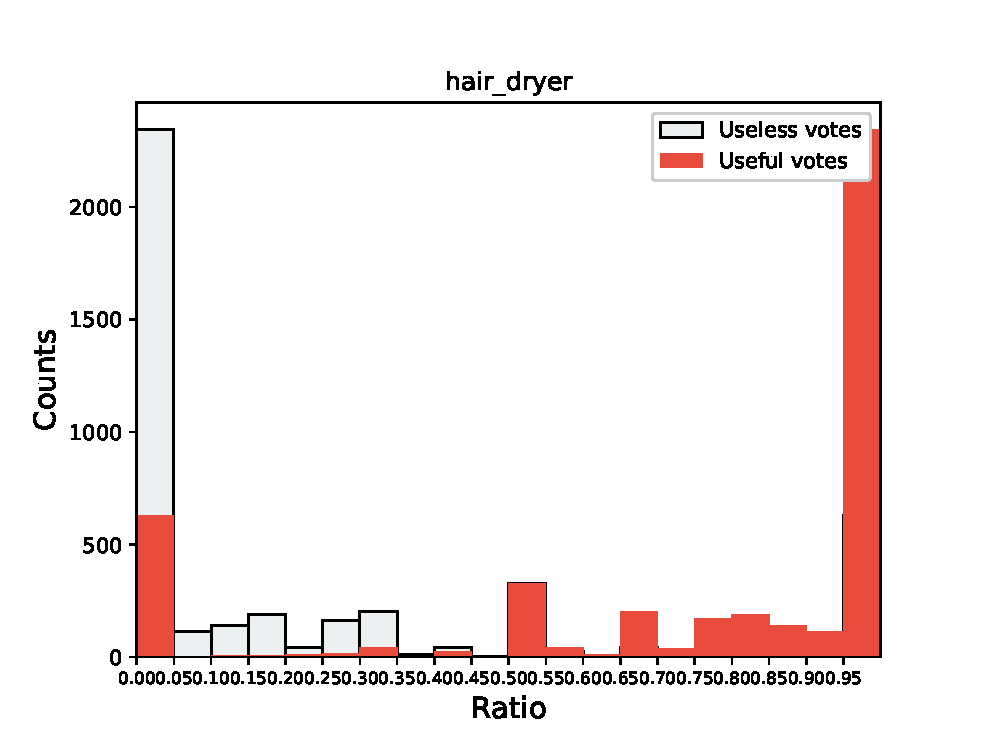
\includegraphics[scale=0.3]{figures/useful_ratio_hair_dryer.eps}}
    \subfigure[Microwave]{
    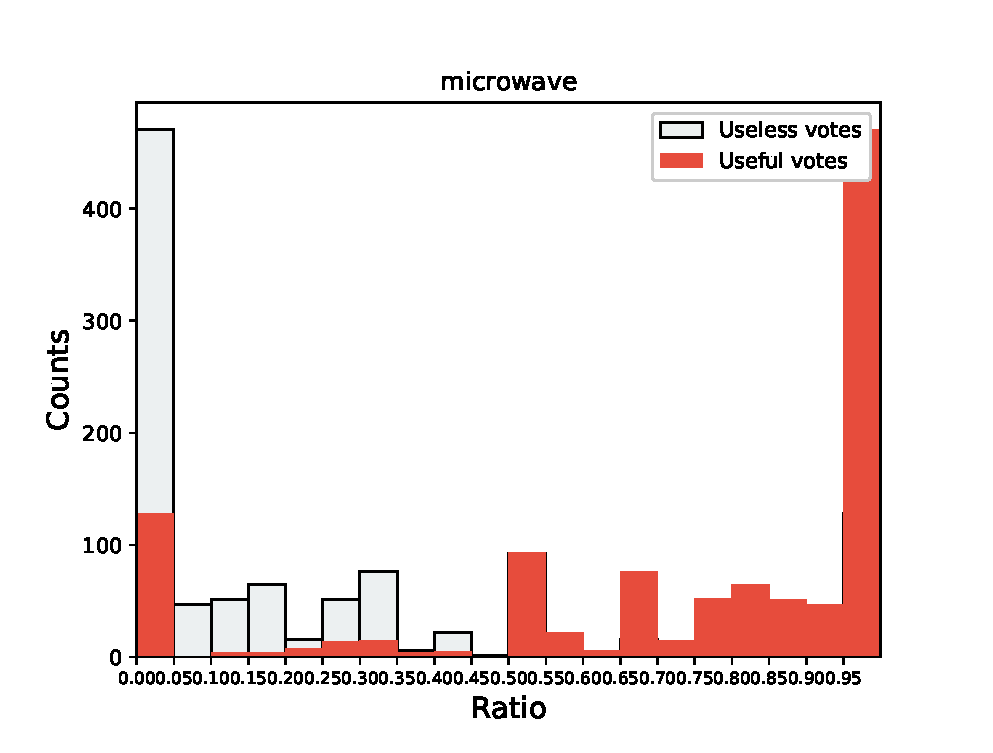
\includegraphics[scale=0.3]{figures/useful_ratio_microwave.eps}}
    \subfigure[Pacifier]{
    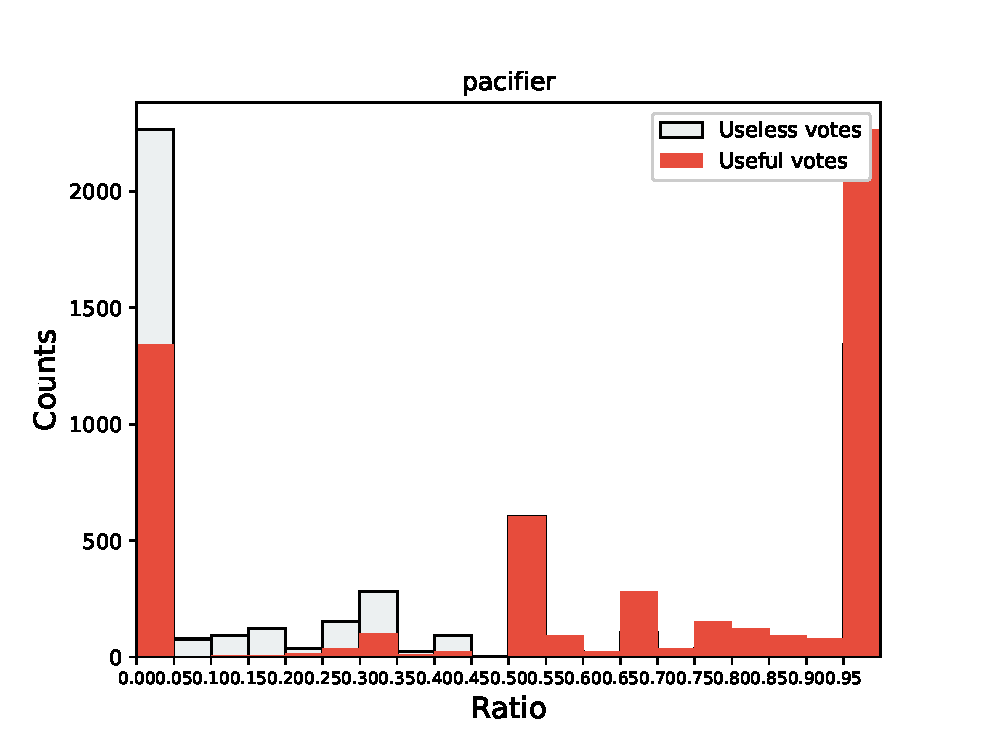
\includegraphics[scale=0.3]{figures/useful_ratio_pacifier.eps}}
    \caption{Ratio of useful votes to total votes}
    \label{fig:ratio_useful}
\end{figure}

After analyzing the data, however, we found most feedback had very little votes. That is to say, these ratio will not be much reliable, and we cannot directly use the ratio as an coefficient. Both of the ratio and the number of total votes have a great contribution to customers' attention.

We find a way to combine the contribution these two dimension. The lower bound of Wilson score confidence interval for a Bernoulli parameter. It was worked out in 1927 by Edwin B. Wilson. \cite{ref:wilson}

$$
p = \frac{\widehat{p}+\frac{1}{2 n} z_{1-\frac{\alpha}{2}}^{2}  - z_{1-\frac{\alpha}{2}} \sqrt{\frac{\widehat{p}(1-\widehat{p})}{n}+\frac{z^2_{1-\frac{\alpha}{2}}}{4 n^{2}}}}{1+\frac{1}{n} z_{1-\frac{\alpha}{2}}^{2}}
$$

In this formula, we can consider $\hat{p}$ is the helpfulness rate, $n$ is the number of total votes. There is a 95\% chance that the 'real' fraction of positive ratings is at least the result of the above formula when $z_{1-\frac{\alpha}{2}} = 1.96$.

This model cannot handle the situation where the feedback has no vote ($n=0$), thus a large amount of feedback cannot be evaluated if we do nothing but ignore this case. To solve this, we consider everyone will vote "useful" for their own review.  That is to say, we can plus one to the 'helpful\_vote' and 'total\_vote' of each feedback. After the transformation, we can use Wilson score confidence interval to determine a number between $0$ and $1$, representing the "credibility" of feedback, that is the ratio $F_U$.


\begin{figure}[ht]
    \centering
    \subfigure[Hair dryer]{
    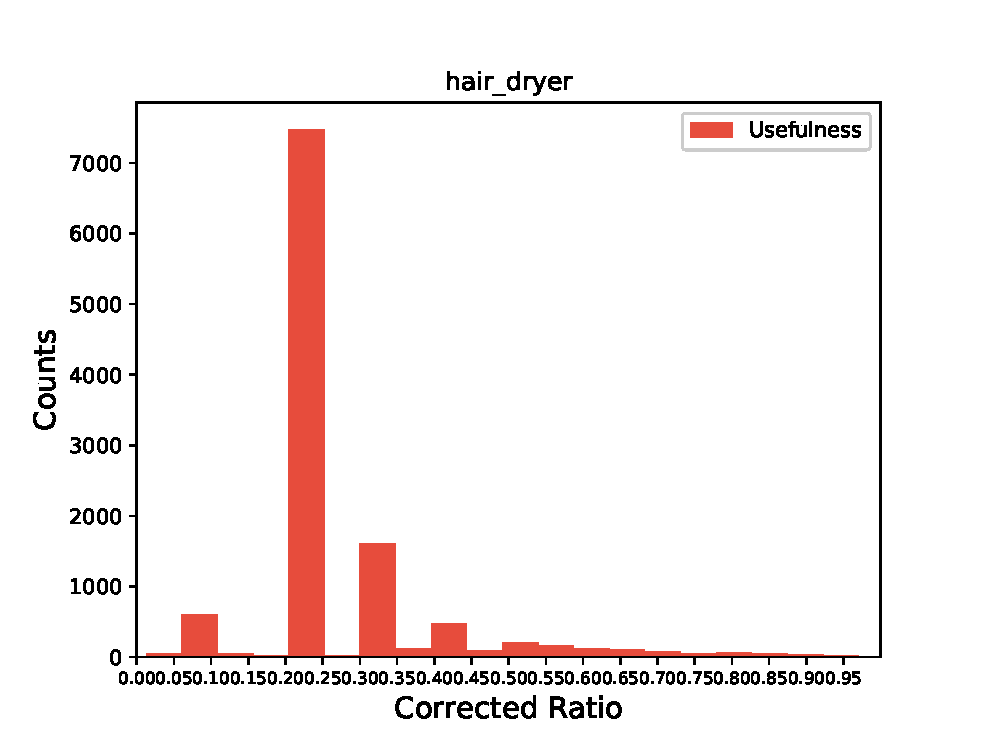
\includegraphics[scale=0.3]{figures/useful_ratio_hair_dryer_new.eps}}
    \subfigure[Microwave]{
    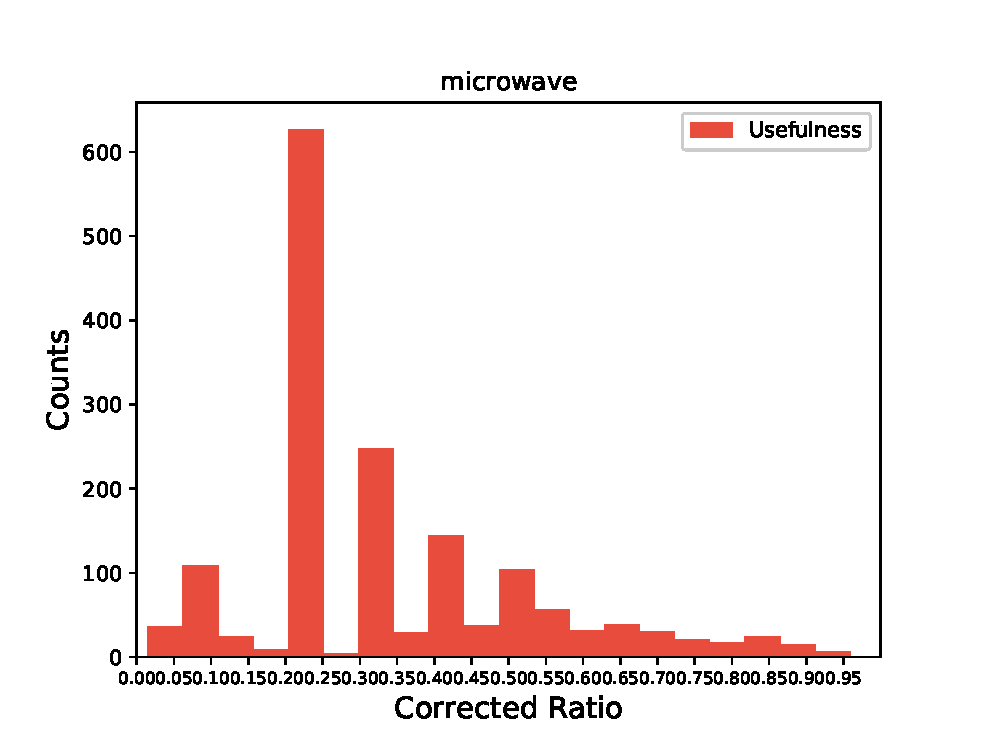
\includegraphics[scale=0.3]{figures/useful_ratio_microwave_new.eps}}
    \subfigure[Pacifier]{
    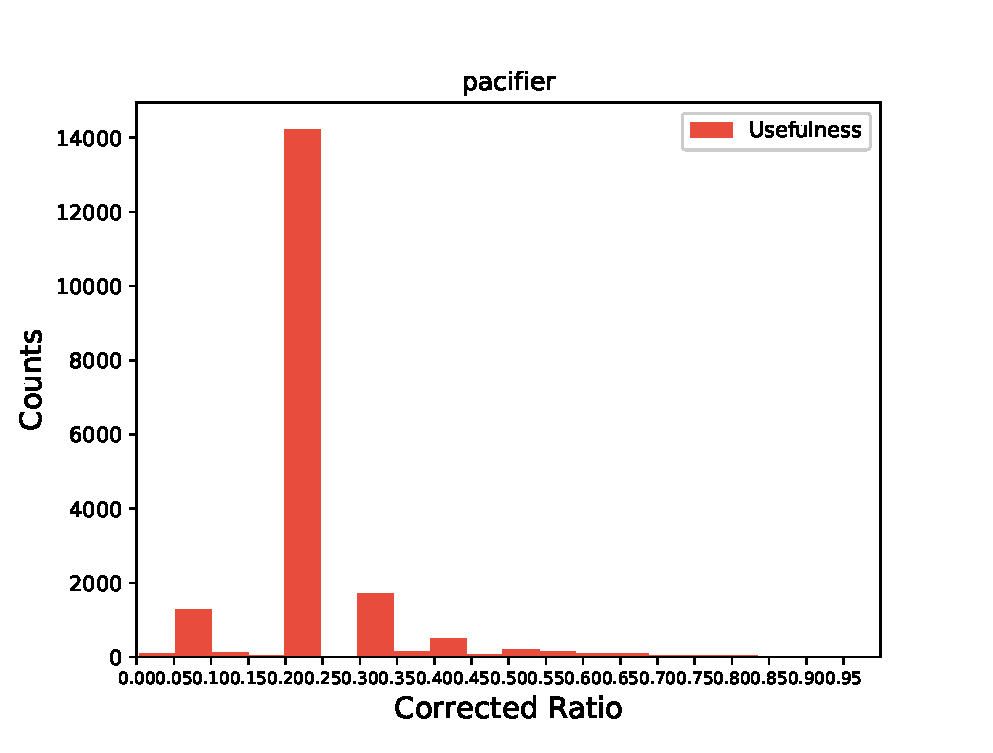
\includegraphics[scale=0.3]{figures/useful_ratio_pacifier_new.eps}}
    \caption{Distribution of Usefulness Ratio $F_U$}
    \label{fig:new_ratio_useful}
\end{figure}


It's more convincing yet doesn't lose too much information about the product. With this assumption, we can consider the impact of the number of votes and the approval rate in the text message.

\subsection{Normalize Length}\label{length}
\begin{figure}[ht]
    \centering
    \subfigure[Raw Word Number]{
    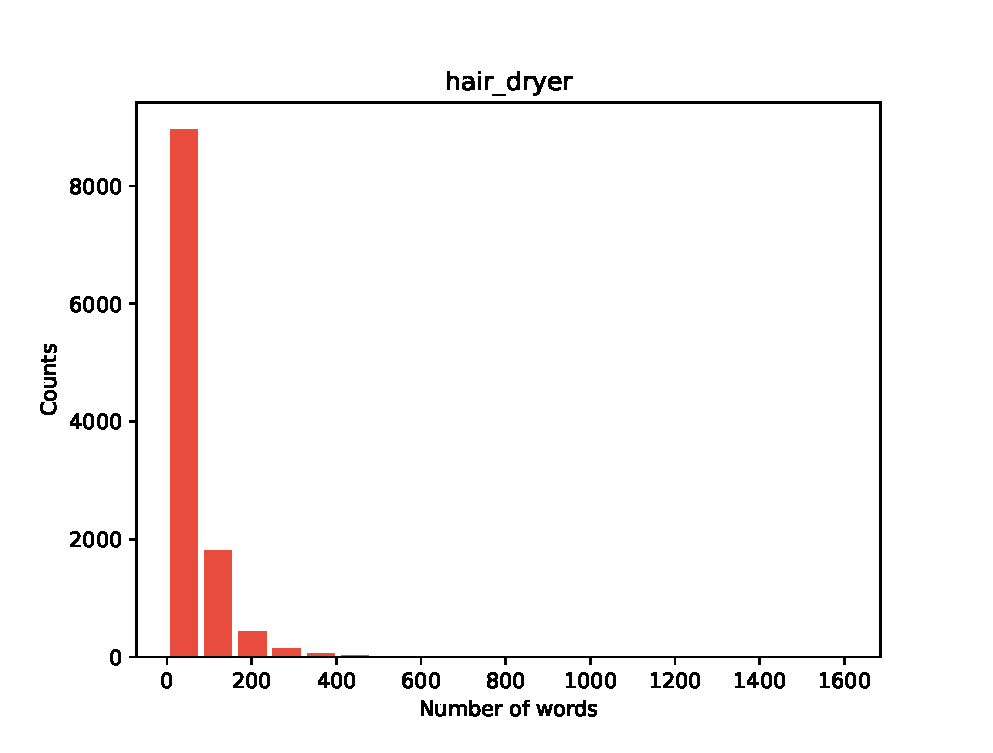
\includegraphics[scale=0.4]{figures/length_hair_dryer.eps}}
    \subfigure[Normalized Length]{
    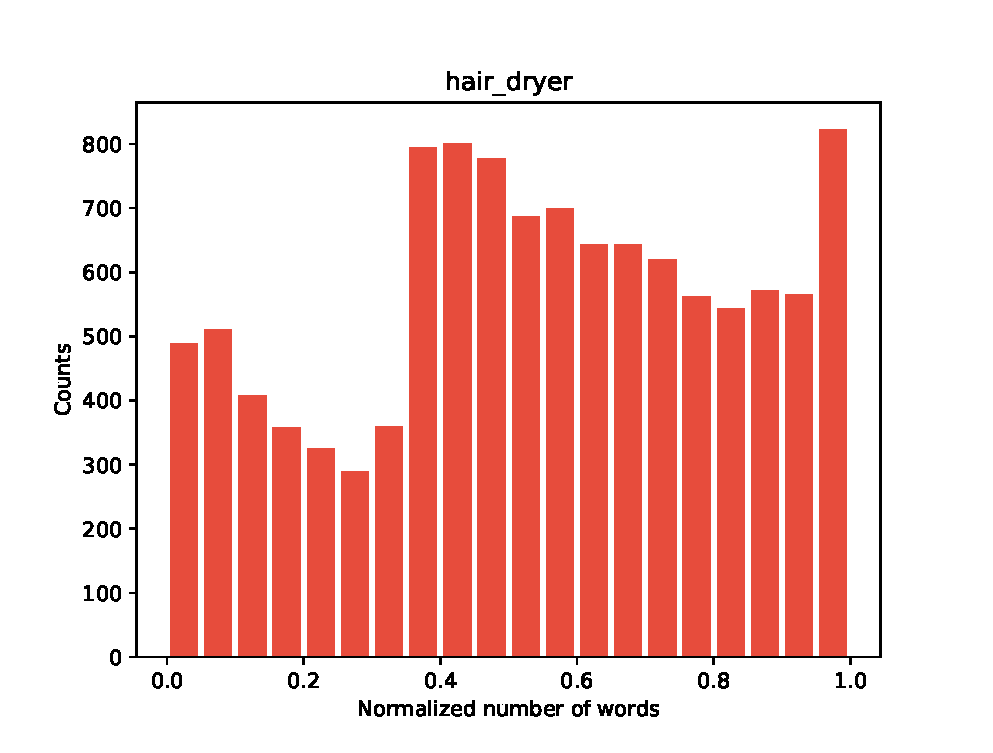
\includegraphics[scale=0.4]{figures/length_hair_dryer_new.eps}}
    \caption{Distribution of Length Data}
    \label{fig:length_pic}
\end{figure}
We take products of hair\_dryer as an example. First we draw a frequency histogram of numbers of words in reviews. And we notice that a linear scale can not describe the influence accurately. We want that the length value to be between zero and one and the function should be increasing and convex. We thought the function$$\widehat R_L = 1 -\frac{1}{\quad e^{R_L/c}}$$ can describe the relation where c is a constant. Then in order to determine the critical value of $c$, we have several trials and finally decided to take $c$ = 50. The frequency of normalized length is as figure 3(b). That is to say we take $$\widehat R_L = 1 -\frac{1}{\quad e^{R_L/50}}$$ as our model.




\subsection{Application of the Model}
We applied the model to three data set respectively. 

For a given feedback, AHP model give a quantitative result which represents the credibility of a feed back. Since weight vector $W$ is
$$
W = 
\begin{bmatrix}
0.2858 \\ 0.0475 \\ 0.0755 \\ 0.4210 \\ 0.1708
\end{bmatrix}
$$
Now we define the corresponding value from 0 to 1 of the five weight :

$h_1$:the value of $\widehat F_U$

$h_2$:the value of $\widehat R_L$

$h_3$:1-$R_S$

$h_4$:the value of $V$

$h_5$:the value of $P$\\
If we define$$
H = 
\begin{bmatrix}
h_1\\h_2\\h_3\\h_4\\h_5
\end{bmatrix}
$$
Then we attach the weight to the corresponding value, $W^T\cdot H$ represents the comprehensive credibility of a feed back.

And we decided star rating and review accounted for 60\% and 40\% respectively. Define and normalize the value of a piece of review is $R_P$ and the value of a star rating is $ \frac{S-2.5}{2.5}$ so that both of them value from -1 to 1. Then a total value represents the evaluation of a feedback is $$(0.6R_P+0.4\frac{S-2.5}{2.5})W^T\cdot H$$

\section{Applications of the Model}
\subsection{Screening of high value review}
After we got an "credibility score"($W^T \cdot H$) for every feedback with analytical hierarchy process, we rank the "uesfulness score" from high to low and make a list of top 10 pieces of review as Table 1\~3 in appendix C. The selected review should be important to companies since high value review have a stronger influence on the other customers. 




%挑选出的高价值的评论
\subsection{Analyzing the results based on time}
As for Sunshine Company's detailed requests, we should apply the model we constructed and analyze the results based on time. To make the results comparable and representative, we choose three products of different product's parent whose total vote number are largest.The product\_id of three products we choose are B003V264WW in Hair dryer, B0052G14E8 in Microwave, B003CK3LDI in Pacifier.
\subsubsection{Discuss the reputation trend of a product}
We want to discuss the reputation trend of the three chosen products. In another word, whether their reputation is increasing or decreasing over time. A product's reputation can be measured by our evaluation model. And take time as variable, a product's reputation can be seen as a function over time. According to the real life product evaluation method, we take the average of all feedback before time t as the estimated reputation at time t. Then we get figures which estimate theses three products' reputation over time. The figures are as follows:

\begin{figure}[ht]
    \centering
    \subfigure[Hair dryer]{
    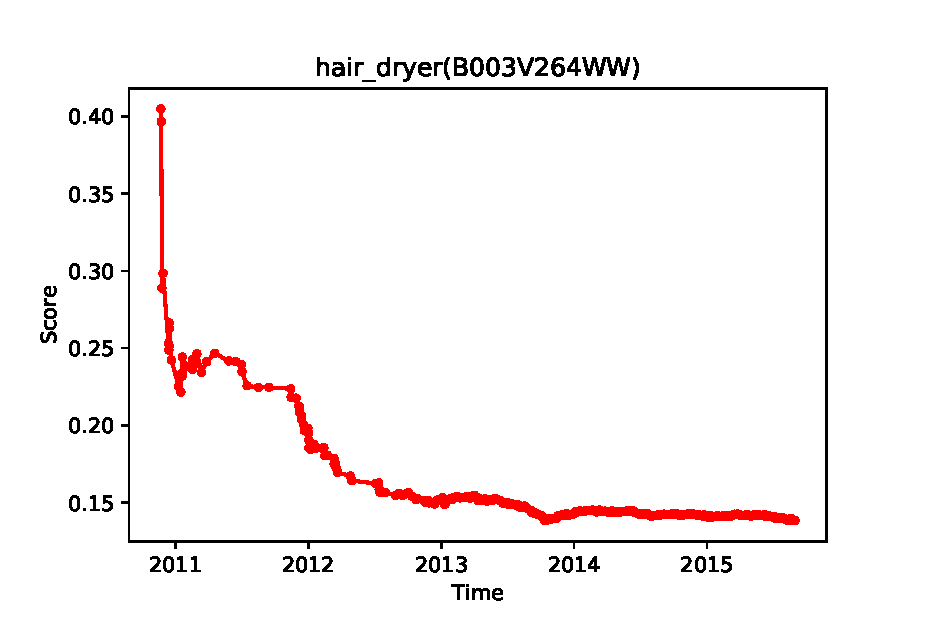
\includegraphics[scale=0.3]{figures/time_hair_dryer.eps}}
    \subfigure[Microwave]{
    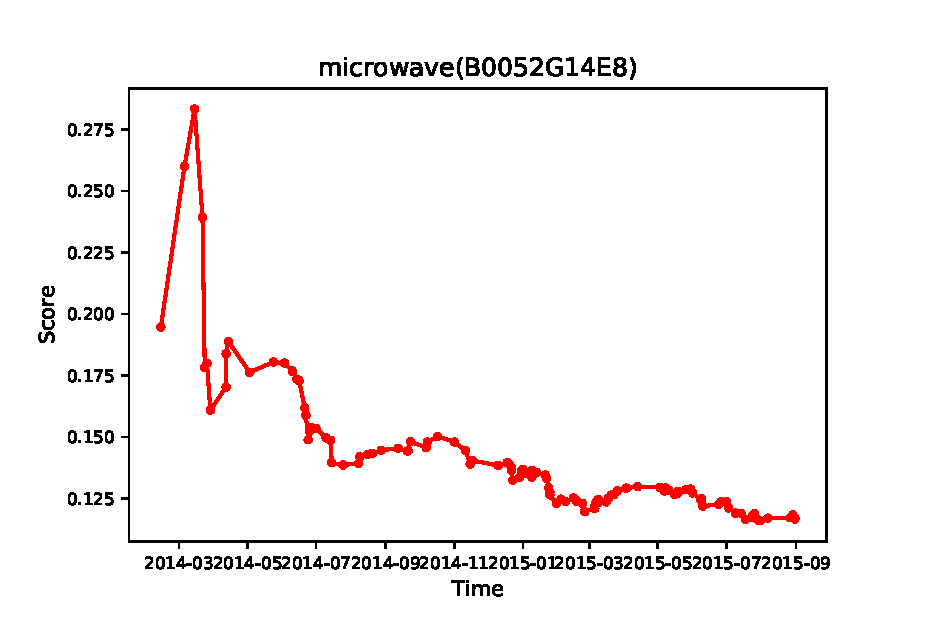
\includegraphics[scale=0.3]{figures/time_microwave.eps}}
    \subfigure[Pacifier]{
    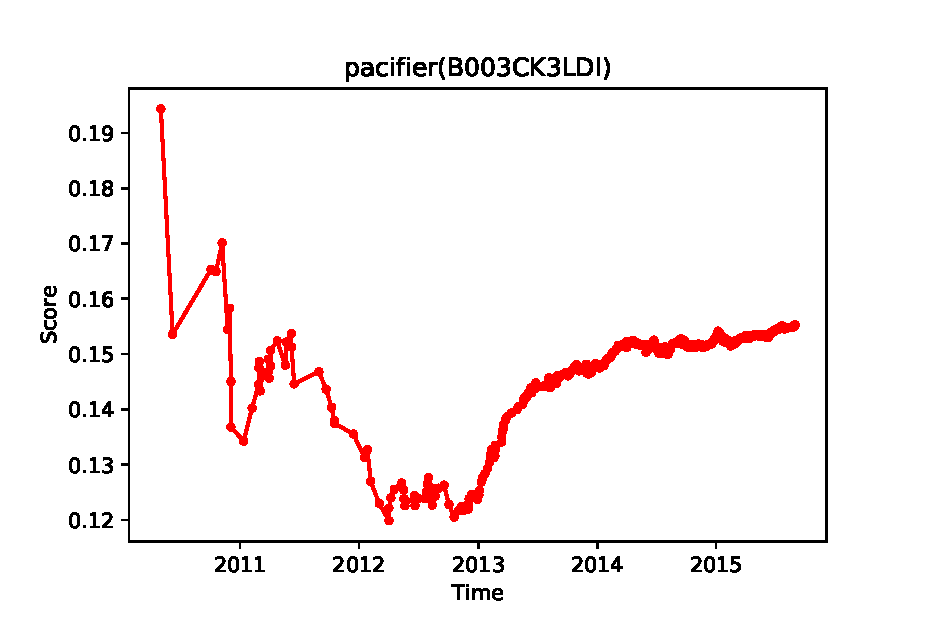
\includegraphics[scale=0.3]{figures/time_pacifier.eps}}
    \caption{estimated trend of three representative product}
    \label{fig:p_trend}
\end{figure}

These figures show that how does the estimated reputation change over time. We can observe their reputation is increasing or decreasing and the sale trend behind it. Clearly a high-valued reputation represents the product has a better or worse sale trend. Moreover, we notice that there is several inflection points in the figures. The estimated reputation behave quite differently in the different side of the inflection point. In general, the first product' reputation is decreasing over time and tends to be stable finally. The second is similar to the first one. But the third one have a upward trend clearly. If we compare there three products, we claim that the first one and third one have a better reputation than the second but the third one has a best sale potential.

\subsubsection{Stars, Length of Reviews, and Amount of Feedback} 
%%begin{\中文区}
%现在我们对特定的星级是否会对引起更多的评论进行讨论。我们认为更多的评论可以从两个方面衡量:其一是更多数量的评论;其二是每条评论的平均词数。我们认为这两个数字都能衡量更多评论这一行为。
Now we are discussing whether a particular star rating range will cause more feedback. We think that "more feedback" can be measured in two ways: one is an increasing number of feedback; the other is the average number of words per review. We think both of these numbers measure the behavior of more reviews.

If a specific star rating will arouse the user's willingness to comment, then the number of reviews in the month is bound to increase. In addition, we also think that having a higher willingness to comment means that their text comments will be longer.
% 如果特定的星级会对激起用户评论的意愿,那么当月的评论数量势必会增加。此外,我们同时认为具有更高的评论意愿意味着他们的文本评论会更长。因此,在以下的分析中,我们绘制了每个产品自上市以来每个月的平均星级评分-月评论数的关系图。以及月平均星级-评论次数长度的关系图。为了明确变化关系,方便找出内在逻辑关联,我们将月平均星级评分以折线图的形式展现,并将评论数和评论次数以柱状图的形式附加在平均星级变化图上。
Therefore, in the following analysis, we have plotted the relationship between the average star rating and the number of monthly reviews for each product since it was launched. And the graph of monthly average star-review length. In order to clarify the relationship of change and find out the internal logical connection, we display the monthly average star rating in the form of a line chart, and attach the number of reviews and the number of reviews to the average star change chart in the form of a bar chart.

% 从众多产品中,我们挑选了 B003CK3LDI这款产品作为示例。虽然这只是是一种产品,并不一定具有普适性,但在我们对每一个产品做同样的分析后发现,图像具有大致相同的规律。以B003CK3LDI这款产品为例的图像如下:
%
From many products, we have selected B003CK3LDI as an example. Although this is just a product, it is not necessarily universal, but after we do the same analysis on each product of different product\_parent, we find that the images have roughly the same rules. Taking the product B003CK3LDI as an example, the image is as follows:
%end{\中文区}

\begin{figure}[ht]
    \centering
    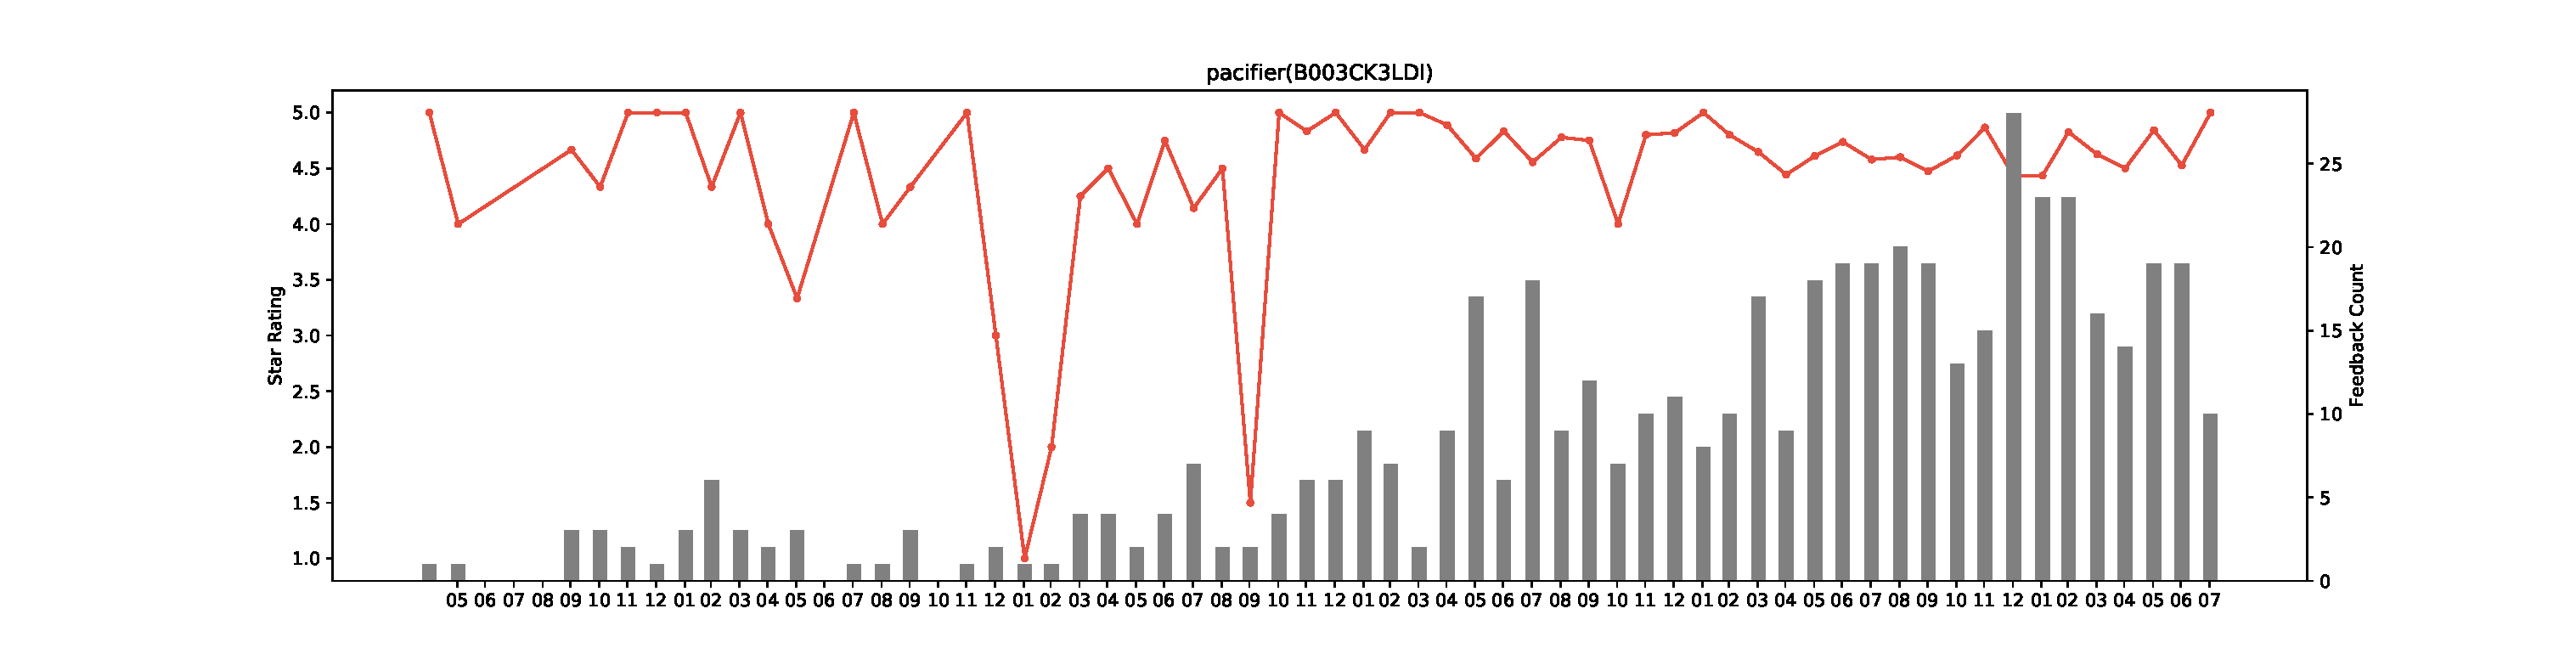
\includegraphics[scale=0.34]{figures/TimeChart/B003CK3LDI_Feedback_Count.eps}
    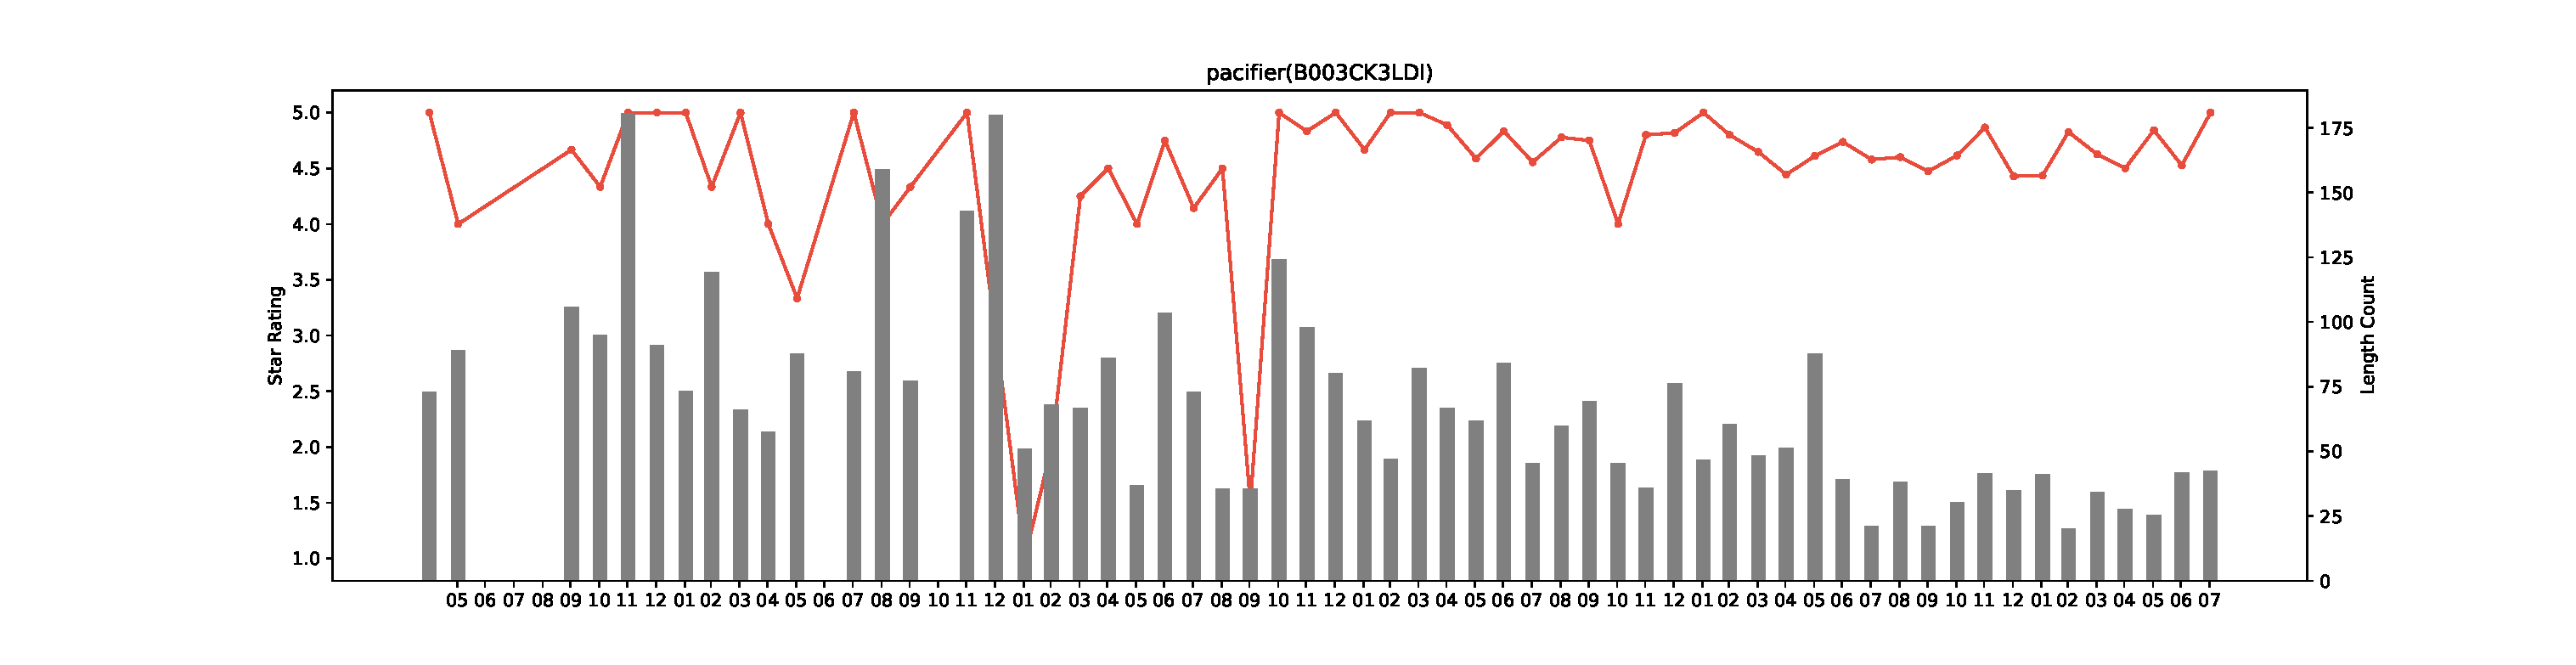
\includegraphics[scale=0.34]{figures/TimeChart/B003CK3LDI_Length_Count.eps}
    \caption{Star Rating and Review Text of Product B003CK3LDI}
    \label{fig:star_review_number}
\end{figure}
We can see that the more pieces of reviews seems to mean the less average of review's words. We thought it is because product reviews tend to stabilize. But we can not know that whether specific star ratings incite more reviews directly from the figure. That is to say, we need to analyze the inner relationship in the following section.



\subsection{The relationship between Star Rating and Review Text}

    It is important to dig into the relationship between star ratings and review text. In our model, we use a naive Bayes classifier to analyze the review text quantitatively. After some conversion, we got the polarity and subjectivity of the review text.
    
    From the perspective of common sense, we think that the polarity of the review text in a piece of feedback is approximately positively related to the star rating. To corroborate this view, we plotted the relationship between polarity and star ratings, and calculated their correlation coefficients. The results of the correlation coefficient calculation and the relationship diagram are shown below.
    
    
    \begin{center}
        \begin{tabular}{|l|l|l|l|}
        \hline
                    & hair dryer   & microwave    & pacifier     \\ \hline
            correlation coefficient & $0.49519728$ & $0.57886614$ & $0.44967142$ \\ \hline
        \end{tabular}
    \end{center}
    
    
    \begin{figure}[ht]
        \centering
        \subfigure[Hair dryer]{
        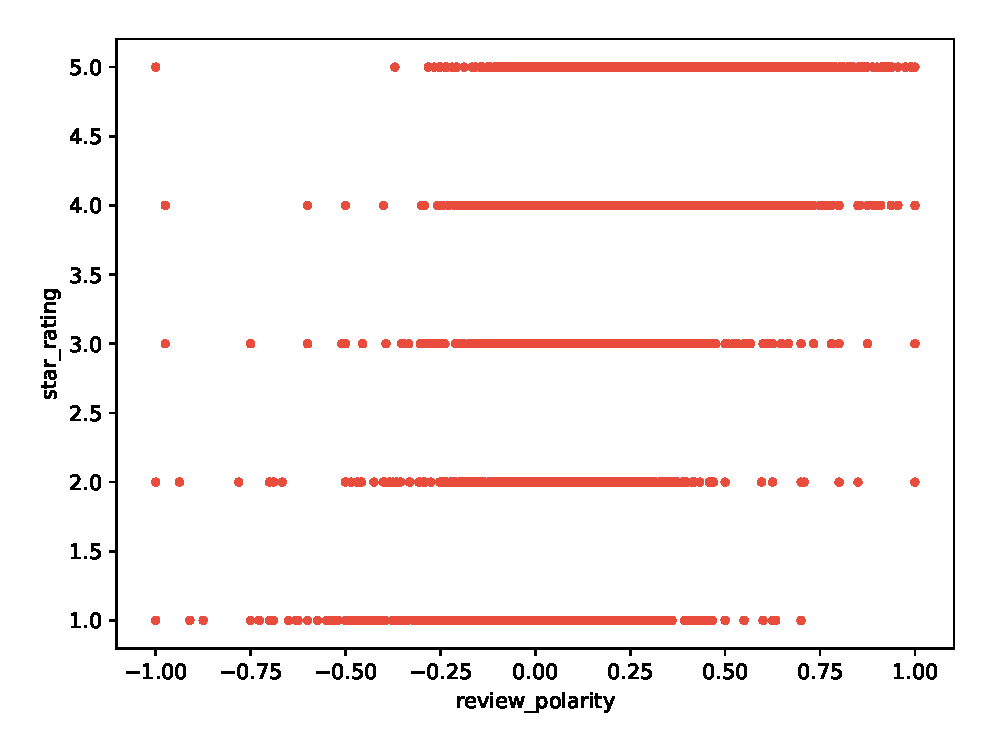
\includegraphics[scale=0.3]{figures/new_hair_dryer_polarity.eps}}
        \subfigure[Microwave]{
        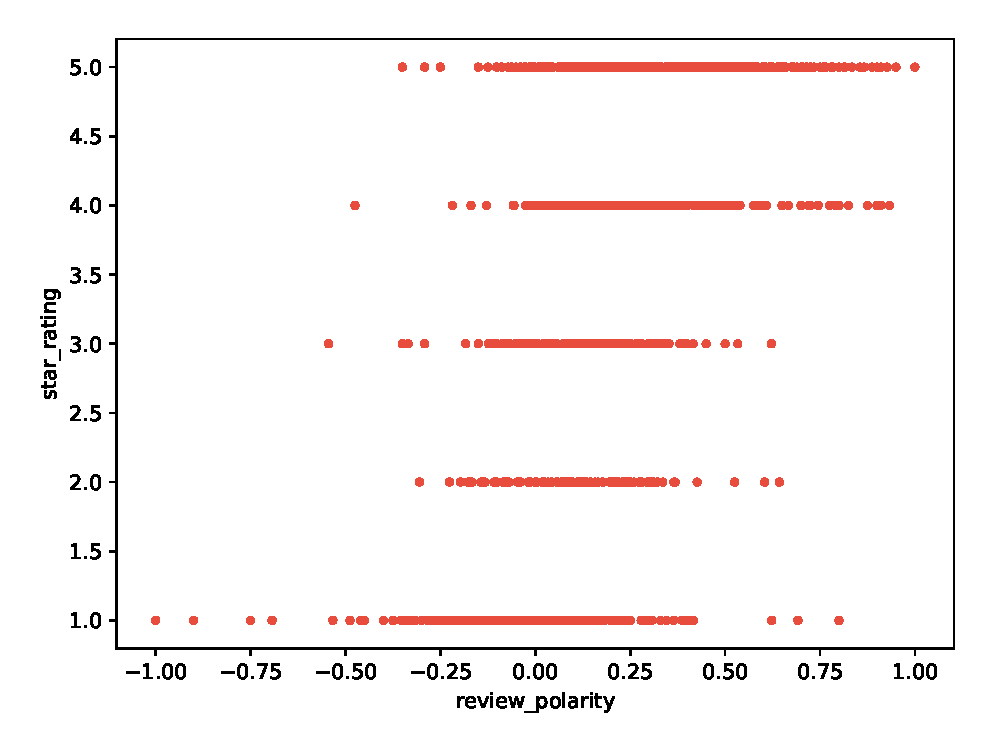
\includegraphics[scale=0.3]{figures/new_microwave_polarity.eps}}
        \subfigure[Pacifier]{
        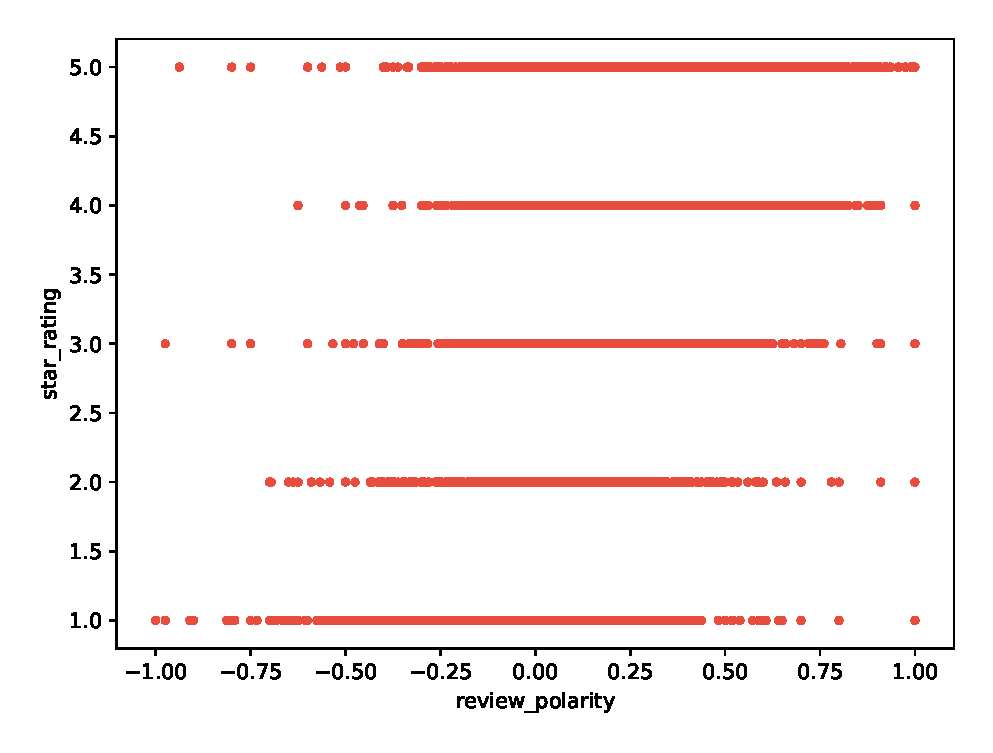
\includegraphics[scale=0.3]{figures/new_pacifier_polarity.eps}}
        \caption{Polarity and Star Rating}
        \label{fig:polarity_star}
    \end{figure}

    In addition, we also care about the relationship between the subjectivity of the review text and the star rating given by the user. Therefore, we use the same method to calculate the correlation coefficient between them and draw the relationship diagram.
    
    \begin{center}
        \begin{tabular}{|l|l|l|l|}
        \hline
                    & hair dryer    & microwave     & pacifier      \\ \hline
            correlation coefficient & $0.17717353$ & $0.27899833$ & $0.15976552$ \\ \hline
        \end{tabular}
    \end{center}
    
    \begin{figure}[ht]
        \centering
        \subfigure[Hair dryer]{
        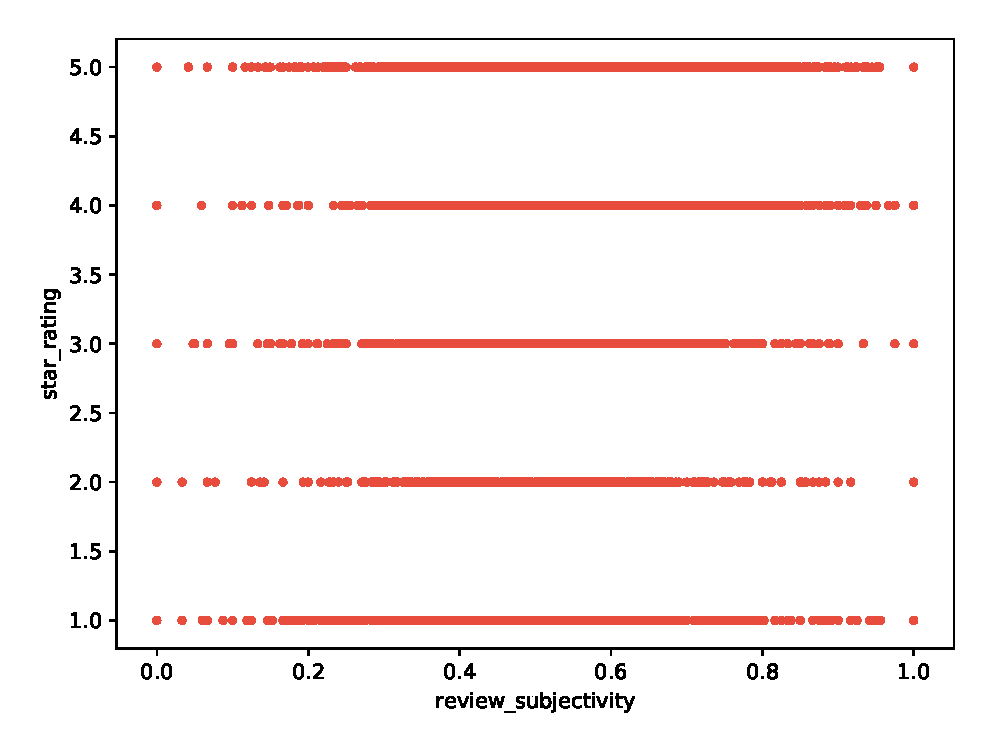
\includegraphics[scale=0.3]{figures/new_hair_dryer_subjectivity.eps}}
        \subfigure[Microwave]{
        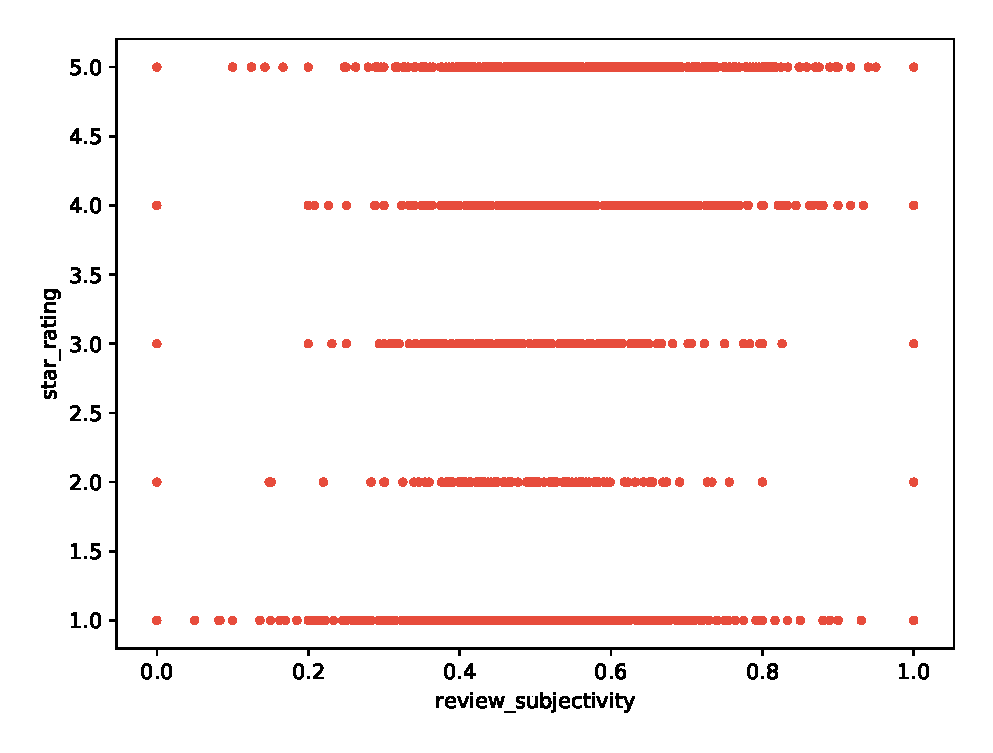
\includegraphics[scale=0.3]{figures/new_microwave_subjectivity.eps}}
        \subfigure[Pacifier]{
        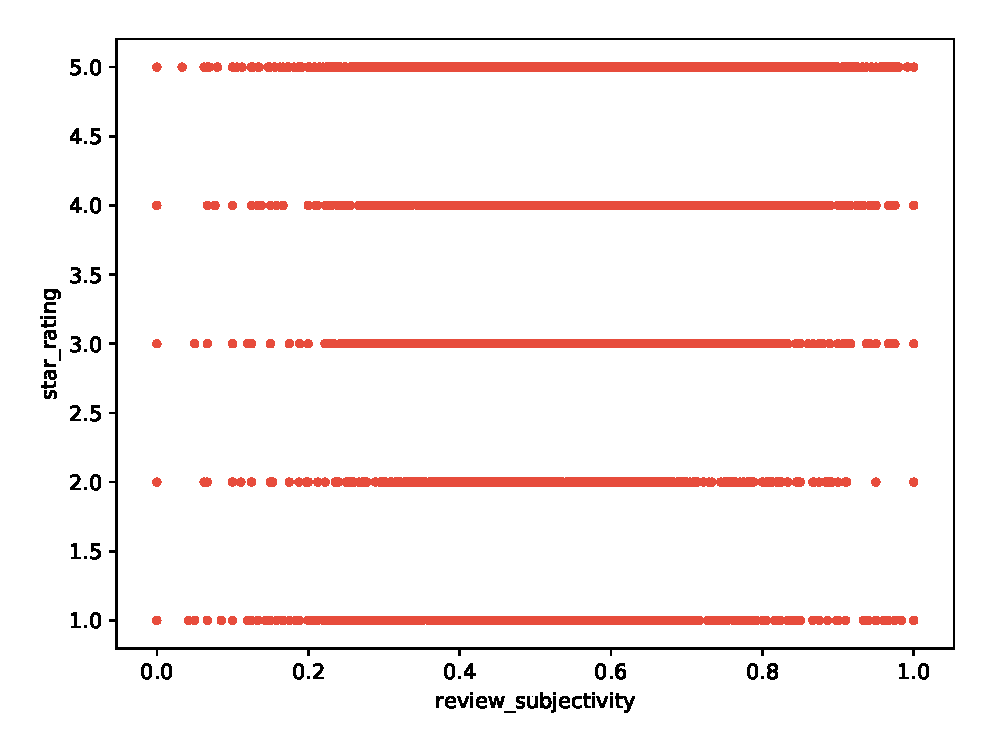
\includegraphics[scale=0.3]{figures/new_pacifier_subjectivity.eps}}
        \caption{Subjectivity and Star Rating}
        \label{fig:subjectivity_star}
    \end{figure}
    
    It can be seen from the pictures and tables that the polarity and the star rating given by the user have a weak positive correlation. However, subjectivity has little to do with star ratings. This is also very reasonable in real life. The emotions of users are directly reflected in the ratings they give, but the subjectivity of their reviews varies. Some users tend to give objective, detailed comments, while others prefer to use words with strong emotions.
    
    To further illustrate the relationship between comments and sentiment and subjectivity in the model we use, we selected a few words and listed the average of star ratings and scores we evaluated to show the ability of out Naive Bayes classifier.
    
    % 此处举例子
    %%一个无处安放的表格
     \begin{center}
        \begin{tabular}{|c|c|c|}
        \hline
             key word    & average star     & average score      \\ \hline
             good & $4.141$ & $0.343$ \\ \hline
             love & $4.688$ & $0.335$ \\ \hline
             happy & $4.363$ & $0.341$ \\ \hline
             useful & $4.264$ & $0.259$ \\ \hline
             bad & $3.235$ & $0.060$ \\ \hline
             hate & $3.530$ & $0.071$ \\ \hline
             useless & $2.420$ & $0.015$ \\ \hline
             angry & $2.870$ & $-0.057$ \\ \hline
        \end{tabular}
    \end{center}
    
    % 我们从评论中挑选了一些明显具有情感倾向的词汇。之后计算了包含这些词汇的评论的平均星级评分和模型给出的综合评分。结果显示,具有明显情感倾向的词语对用户给出的评价有明显的相关性。
    From the review, we picked out some words that were clearly emotionally oriented. The average star rating and the comprehensive rating given by the model were then calculated. The results show that words with obvious emotional tendencies have a significant correlation with the evaluations given by users.
    %
    

\subsection{Attracted feature of these product}
    Based on the credibility evaluation model we have given, we can pick out reviews that are useful for each category and filter out those that are not significantly helpful. Next, we picked reviews with credibility greater than 0.5 ($W^T\cdot H > 0.5$) in each category and plotted the word cloud after proper processing.
    
    We use word clouds to visualize the noun phrases that are repeatedly mentioned in these useful reviews. These noun phrases include the user's intuitive experience after using the product and the most prominent selling point. Making such pictures can facilitate the company's marketing department, allowing them to quickly locate the needs of users, understand the market's concerns, find the value of good products, and improve their products.
    %基于我们给出的feedback usefulness评价模型,我们可以挑选出每个品类具有效用性的评论,并筛除那些显著没有帮助的评论。接下来,我们挑选了每个品类中 usefulness 大于 0.5 的评论,在适当处理后绘制了词云。
    %我们用词云直观地展现这些useful 的评论中反复被提及的名词短语。这些名词短语包括用户使用产品后的直观感受、最突出的卖点和最显著的槽点。制作这种图片能方便公司市场部门,让他们迅速定位用户的需求,了解市场的关注点,找到好产品的价值所在,并改进自家产品。
    
\begin{figure}[ht]
        \centering
        \subfigure[Hair dryer]{
        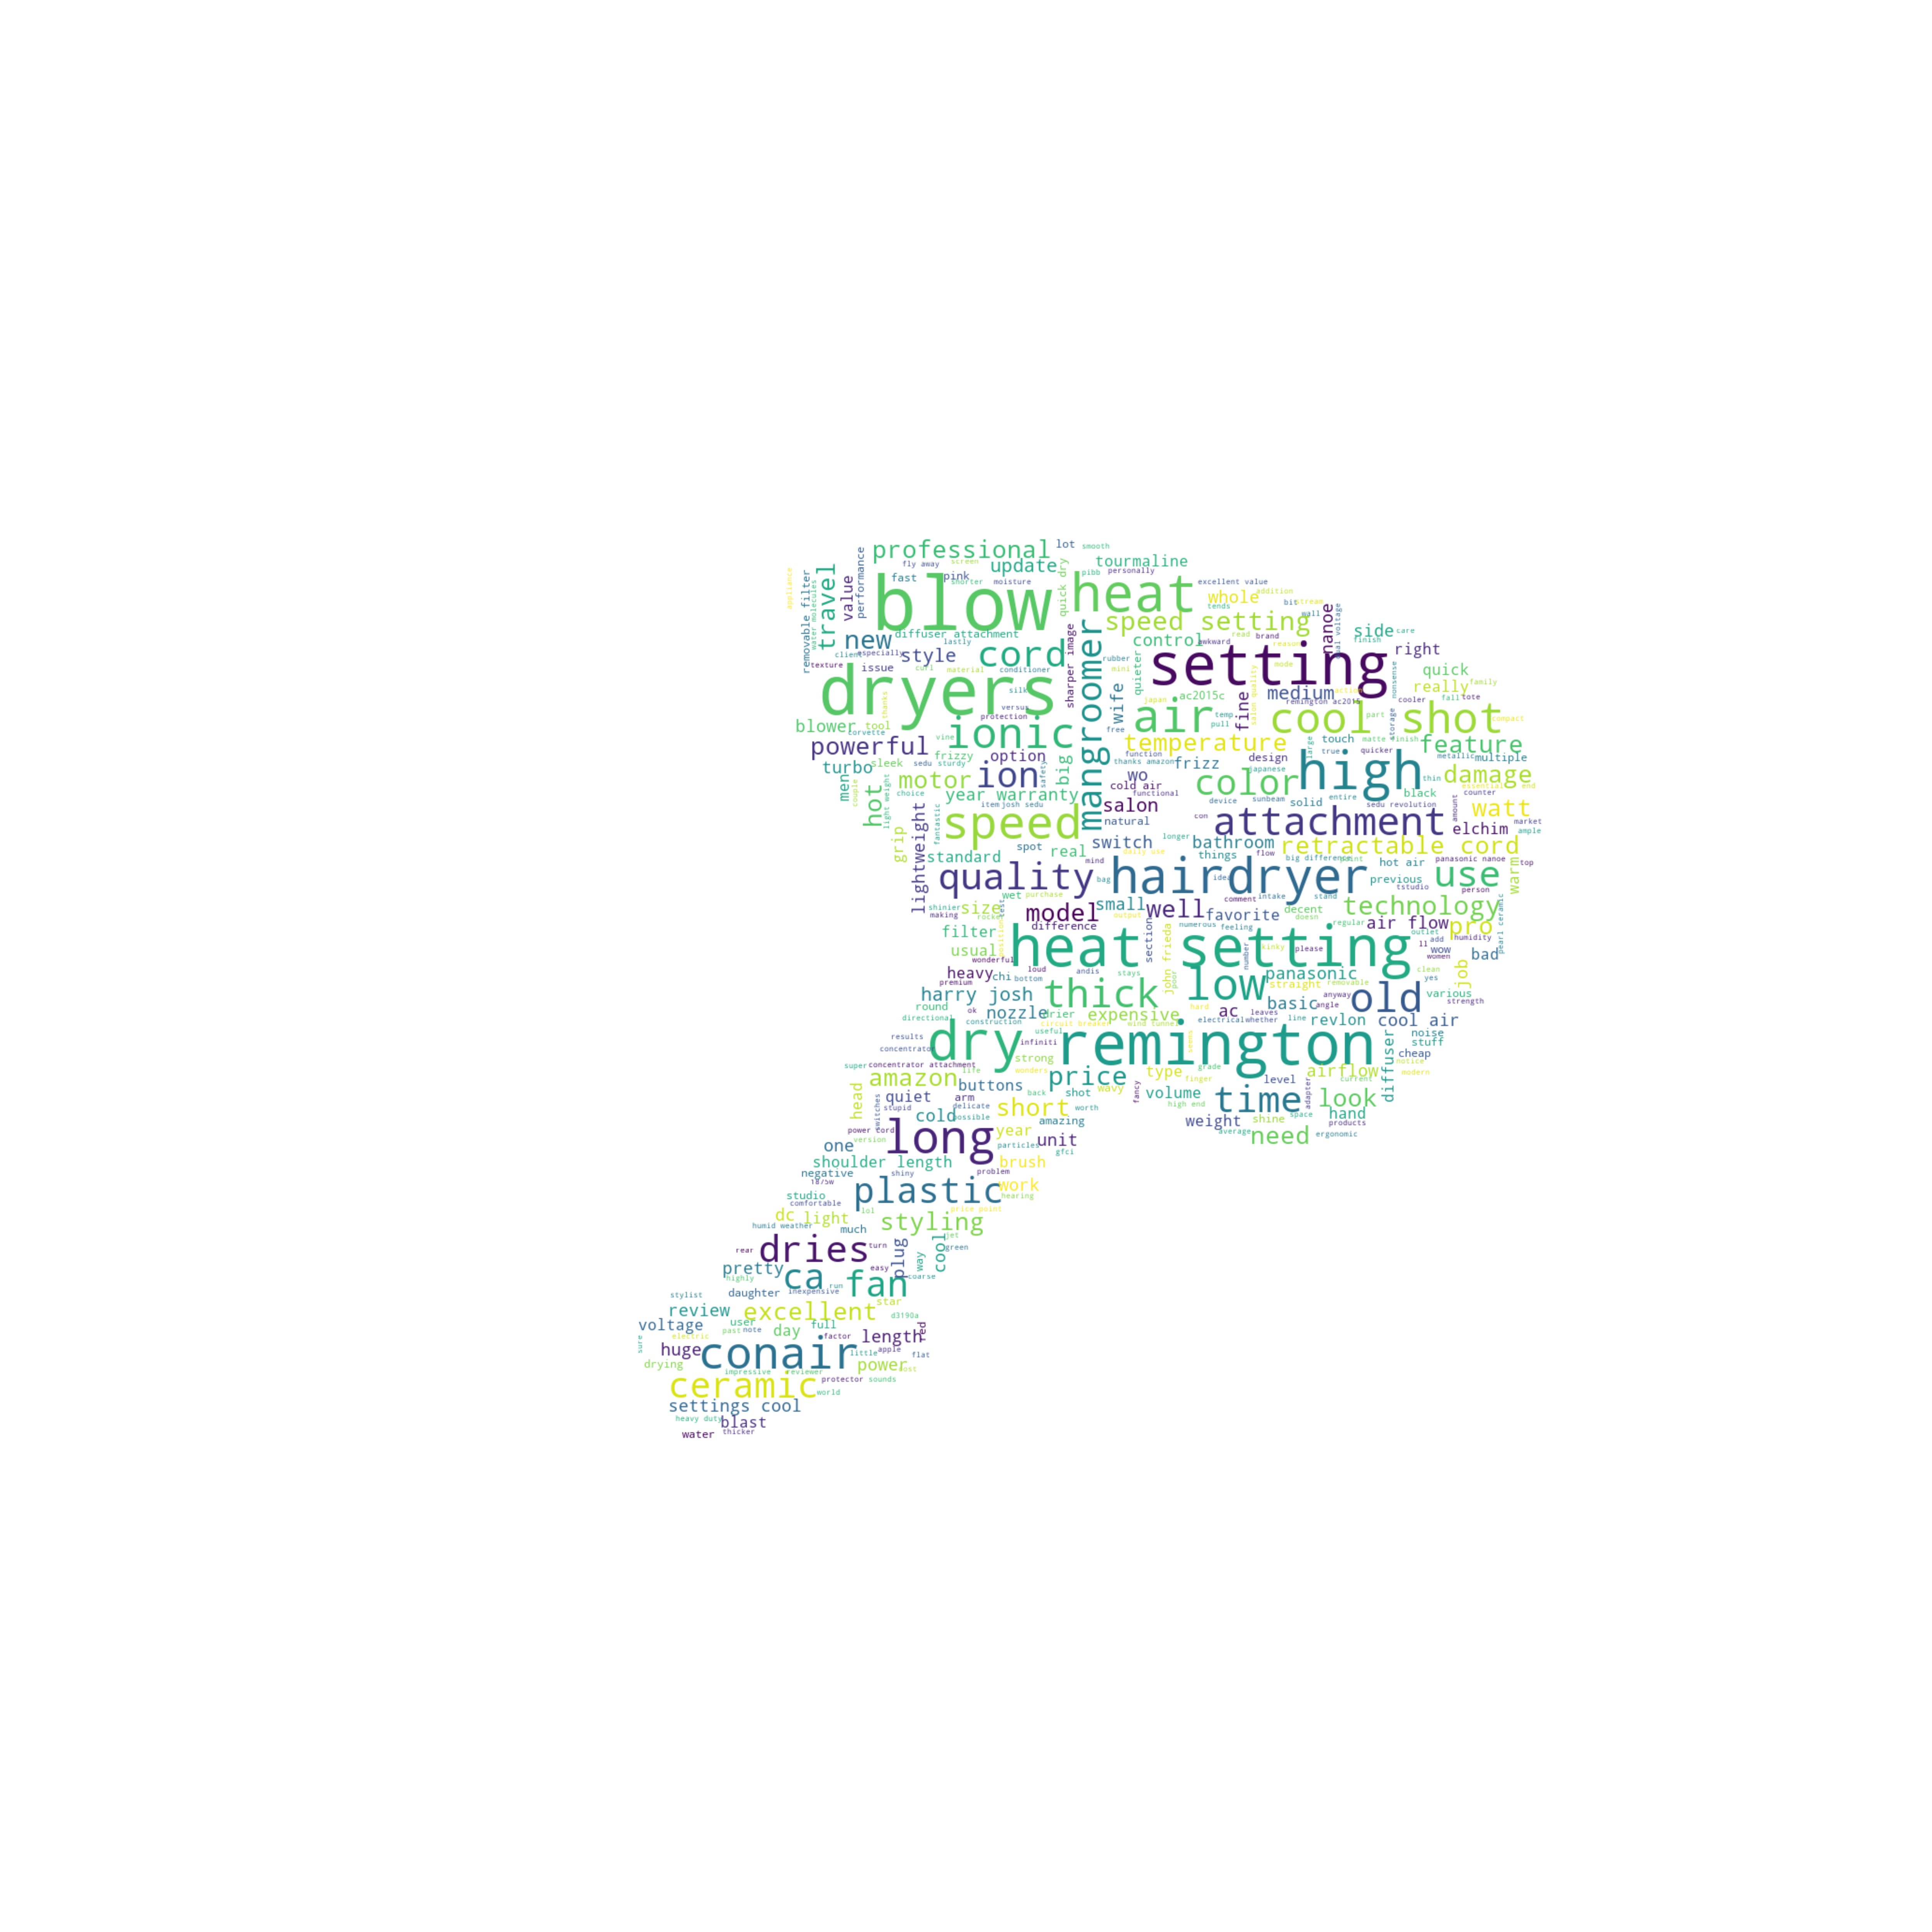
\includegraphics[scale=0.06]{figures/word_cloud/hair_dryer_cloud.png}}
        \subfigure[Microwave]{
        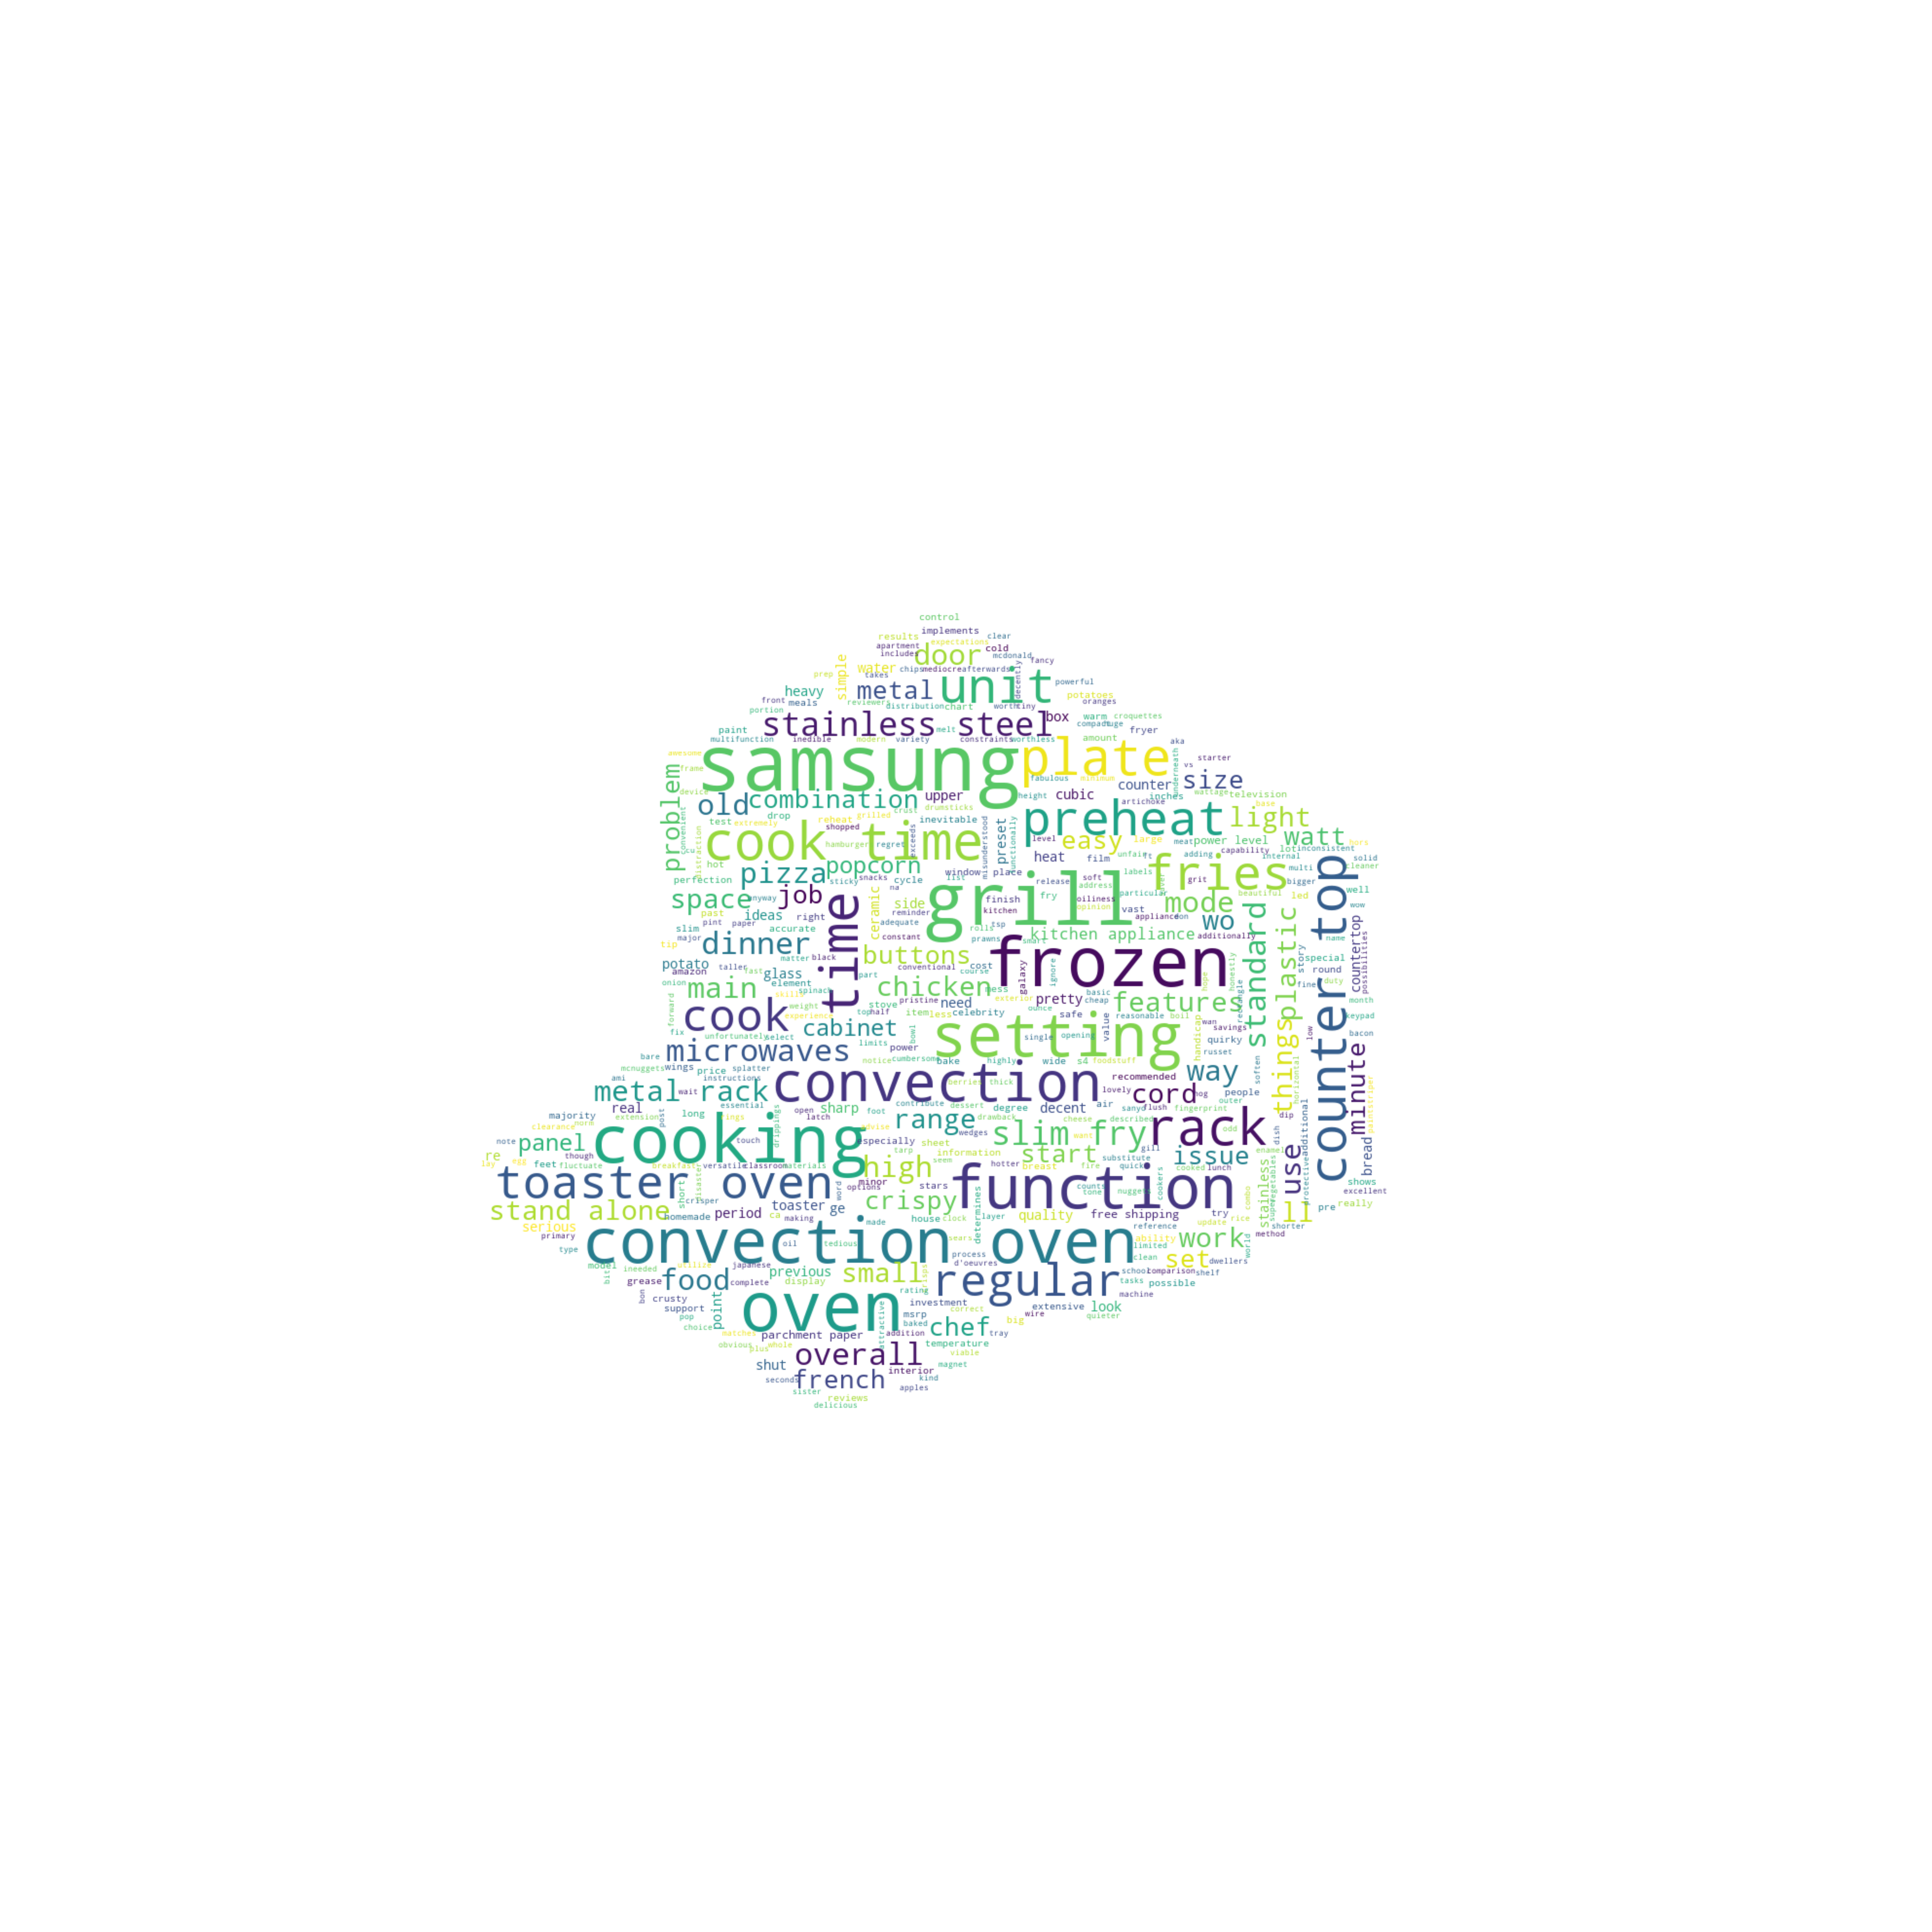
\includegraphics[scale=0.06]{figures/word_cloud/microwave_cloud.png}}
        \subfigure[Pacifier]{
        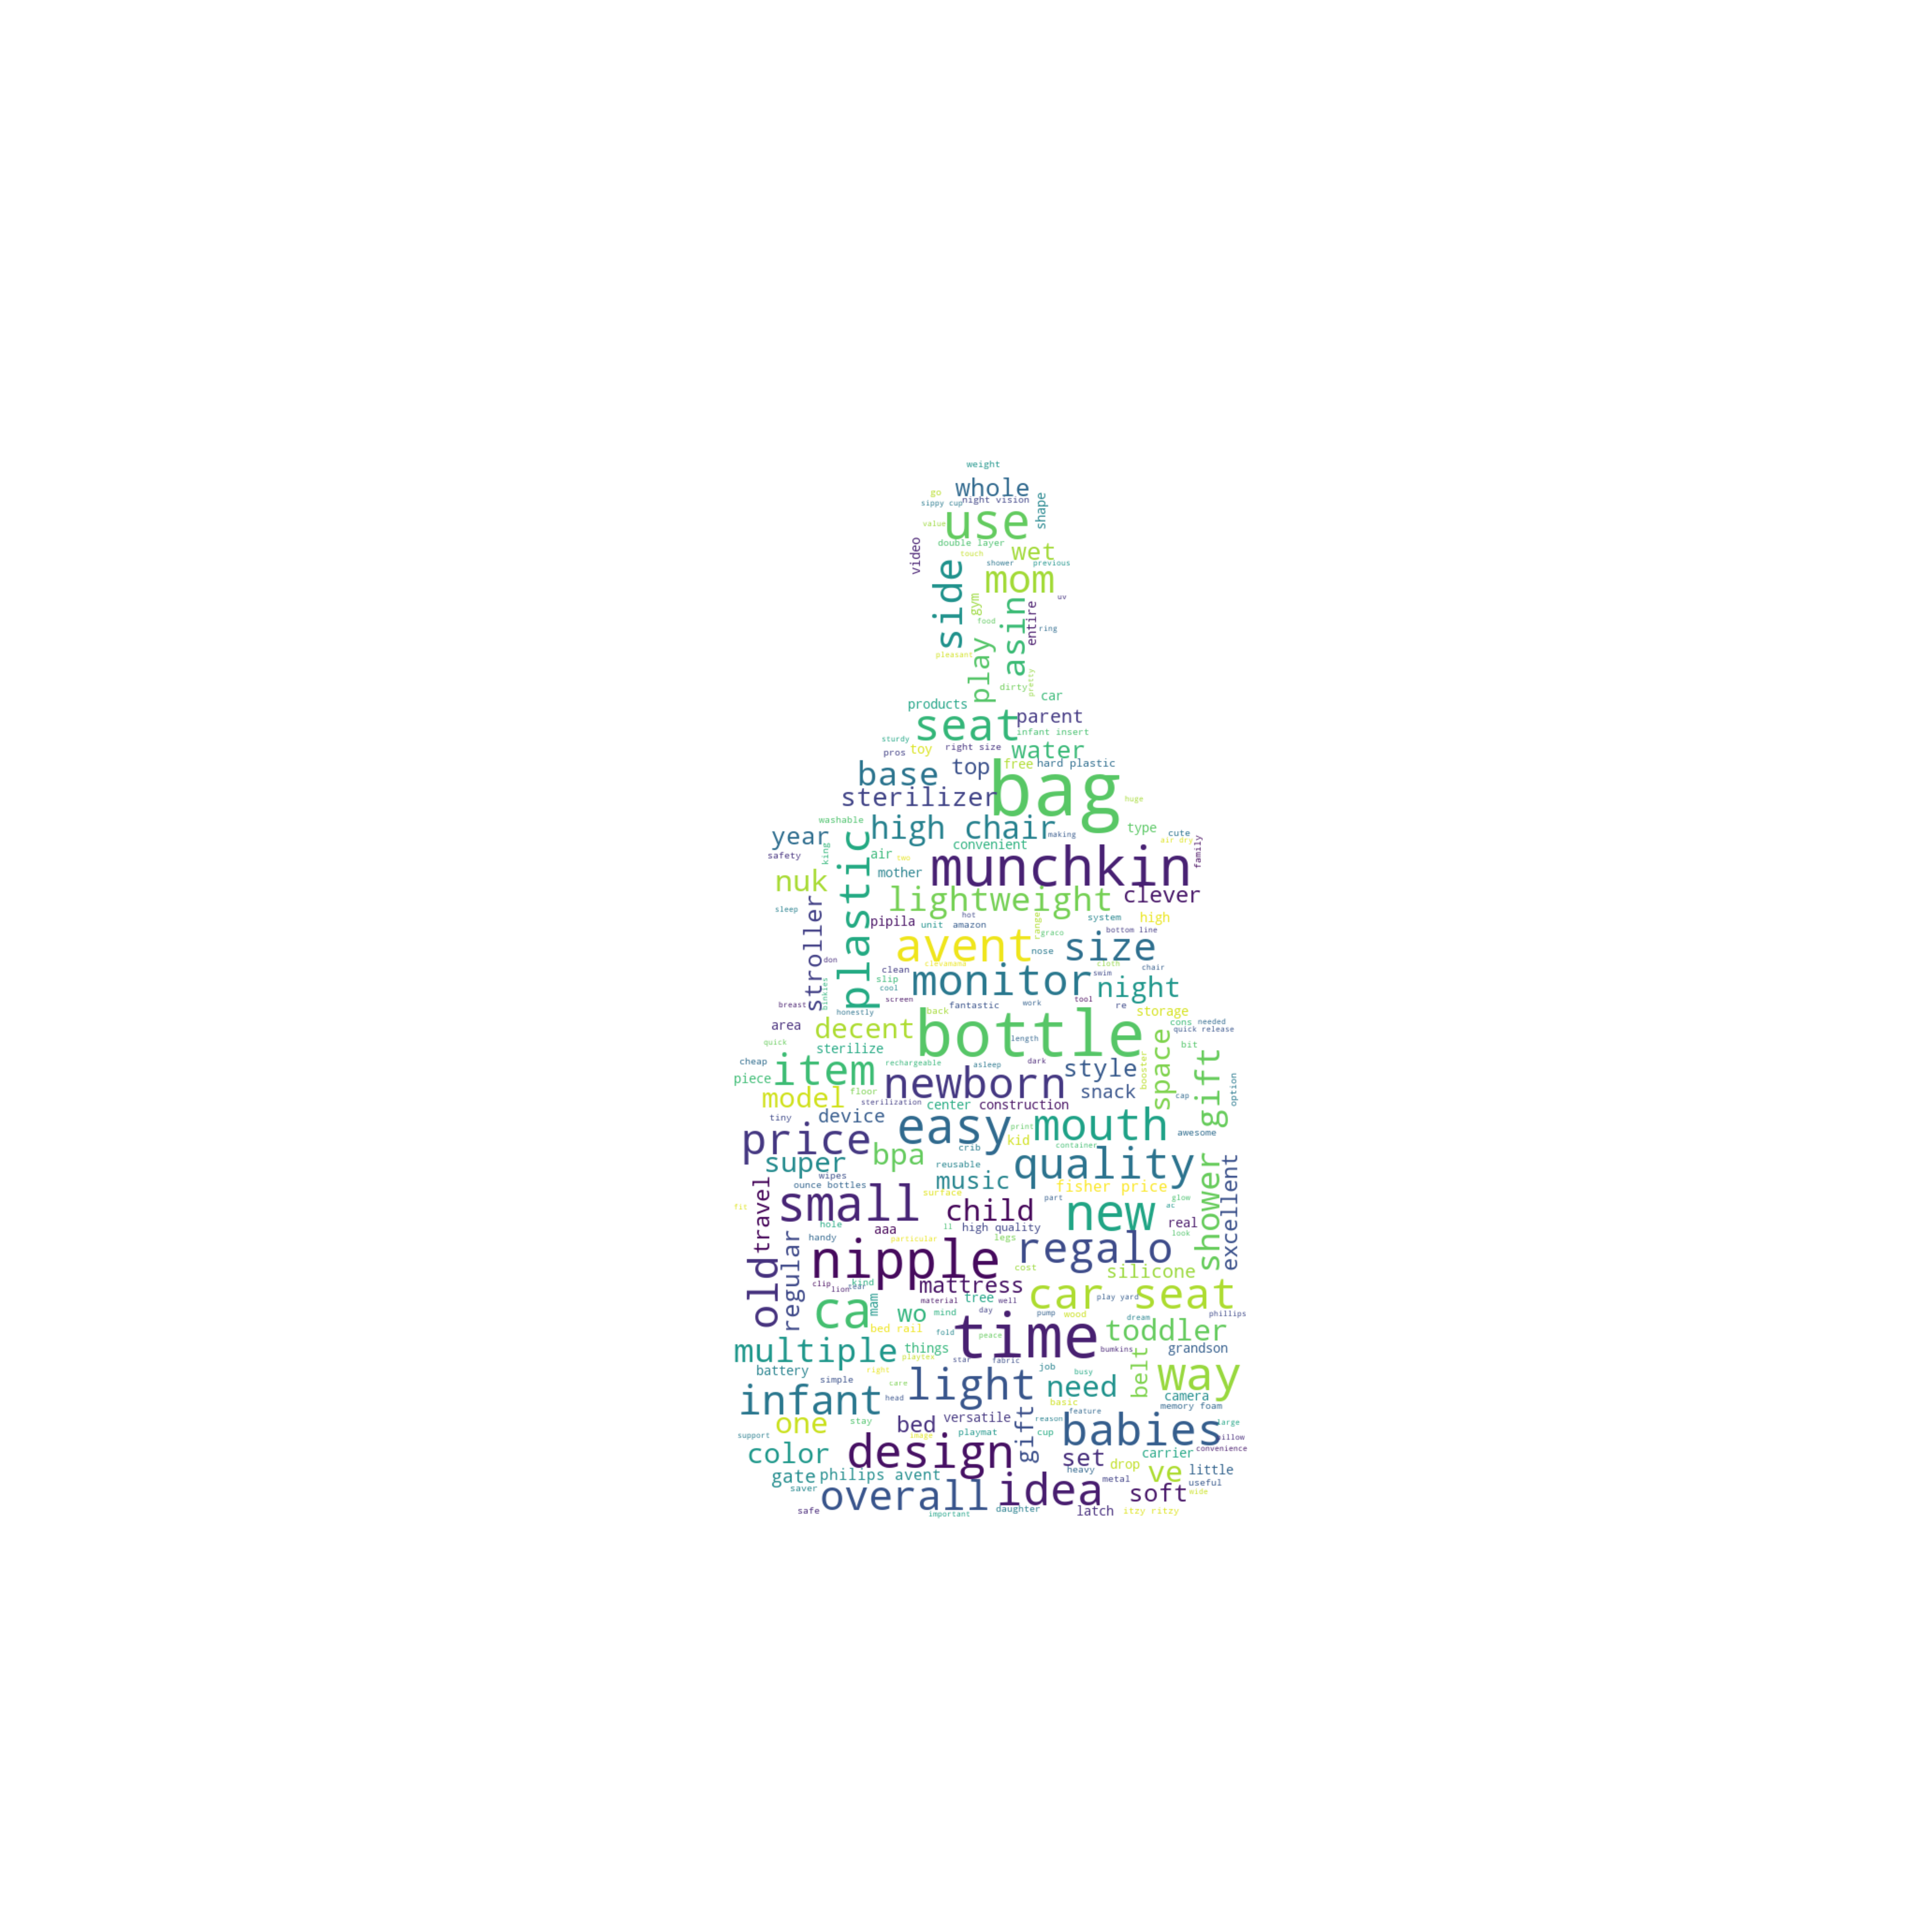
\includegraphics[scale=0.06]{figures/word_cloud/pacifier_cloud.png}}
        \caption{word cloud of three product}
        \label{fig:word_cloud}
\end{figure}


\section{Conclusions}
In this paper, we build a model to analyze the credibility of a review. We use the processed data and grade a piece of review on five factors.According to the model, we can find out reviews that influence other customers the most. And we rated the credibility of a product's review from high to low and identify check the model for practicality.

We also build a model which can give a quantitative result to measure a product's reputation as well as its sale trend.We selected three representative products of different product parent. We apply our model to selected products and analyze their reputation trend and sale potential with the help of figures.

Finally we discussed the relationship between star rating and review text. The results are very much in line with the actual situation: there is a weak positive correlation between star rating and the polarity of reviews. But there is no correlation between star rating and the subjectivity of reviews. We selected several words with strong emotion and found that reviews containing these words also have a tendency to score high or low.

\begin{thebibliography}{99}%%今天我引用了两篇上个世纪的文献,我真棒 世界级建模!
    \bibitem{ref:AHP}Saaty, T. L. (1988). What is the analytic hierarchy process?. In Mathematical models for decision support (pp. 109-121). Springer, Berlin, Heidelberg.
    
    \bibitem{ref:wilson} Wilson, E. (1927). Probable Inference, the Law of Succession, and Statistical Inference. Journal Of The American Statistical Association, 22(158), 209-212. doi: 10.1080/01621459.1927.10502953
    
    
\end{thebibliography}
    
\newpage

\section{A Letter to Sunshine Company }
    \begin{letter}{Dear Sunshine Company, }
    % With the rapid development of online shopping, nowadays people often choose to buy products from large online sales platforms, such as Amazon. Product companies are also willing to put their products online to increase sales. The biggest feature of online shopping is that customers can choose to leave their own feedback, including star rating and review.
    

    % 网络平台的评论中蕴含了很多信息。然而,大量的信息难以直接解读。因此,需要使用合理的模型进行处理。随着互联网技术的发展,大数据以及云端计算可以给公司关于商品的各种信息。
    There is a lot of information in the feedback on online platforms. However, too much information is hard to read directly. Therefore, a reasonable model is needed for processing data. With the development of Internet technology, big data and cloud computing can give companies all kinds of information about commodities.
    
    % 值得注意的是,除了用户的打分和评论以外,还能从feedback中提取出更多有用的信息。为此,我们使用层次分析法制作了一个多维度的模型,以评判一个feedback的有用程度。这个模型综合了评论的客观性、评论的长度、其他用户对评论的看法、VINE用户的特殊身份、以及用户是否原价购买的信息。通过这个模型,我们可以对商品的所有评价进行排名和过滤,以获得一个更加具有商业价值的商品评论研究数据集。通过这个模型的处理,可以大大减轻企业分析用户评论的工作量。分析产品的工作也变得更加直观。
    
    It's worth noting that in addition to user ratings and review, more useful information can be extracted from the feedback. Therefore, we made a multi-dimensional model by analytic hierarchy processing to judge the credibility of a feedback. The model combines the objectivity of the review, the length of the review, how other other customers look at the review, the special identity of the VINE user, and information about whether the user paid the original price. Through this model, we can rank and filter all the evaluations of commodities to obtain a more commercially valuable commodity review research data set. With this model, the enterprise can greatly reduce the workload of analyzing user comments. The work of analyzing the product also becomes more intuitive.
    
    %为了度量一个产品的声誉变化以及预测他的销售潜力,我们制作了产品声誉与时间的关系图。透过这些关系图,分析产品改进和用户的态度变化的关系将会更加容易。甚至在图像中的拐点位置,可以进一步分析是何种原因造成了这样的拐点。
    To measure changes in a product's reputation and to predict its sales potential, we created a product's reputation versus time graph. Through these diagrams, it will be easier to analyze the relationship between product improvements and changes in user attitudes. You can even further analyze what causes change in the reputation through the image by the inflection point.
    
    
    %我们还分析了评论文本和评论星级之间的关系。我们从两方面考虑评论文本:情感方向以及客观程度。根据对数据的计算,从数学上得到评论星级与文本的情感方向呈弱的正相关关系,而与评论的客观程度无关。因此我们认为,产品的正向的评论文本是可以提高产品的星级水平的。
    
    We also analyzed the relationship between review text and star rating. We consider the review text in two dimension: the emotional direction and the degree of objectivity. According to the calculation of the data, there is a weak positive correlation between the rating of the comment and the emotional direction of the text, but it has nothing to do with the objectivity of the comment. Therefore, we believe that the positive review text of the product can improve the star level of the product.
    
    %%%重拳出击
    %除此之外,为了更好地抽象出一个优秀的产品所具备的更吸引顾客的特质,我们在拟定了一些停用词后对用户评论的文本绘制了基于词频的词云。我们可以很直观地看出顾客真正关心的产品属性(当然这里面很高频的出现了price)
    In addition, in order to better find the more attractive characteristics of an excellent product, we drew word clouds based on word frequency to the text of user comments after some stop words were proposed. We can intuitively see the product attributes that customers really care about (of course, there is a high frequency of price).
    
    %听闻贵公司即将在电商平台发售三款产品,我们衷心祝愿贵公司能够取得成攻。同时,我们希望我们的模型可以帮助贵公司更好地通过这些用户评论对贵公司产品销售状况进行预测。我们认为,在将购物网站的原始数据导入了我们的模型之后,消费者的心理及其预期行为将会更直观地展现在我们面前。有关更多该模型和相关结论的详细信息,请阅读我们的论文。
    We heard that your company is about to release three products on Amazon. We sincerely hope that your company will succeed. At the same time, we hope that our model can help your company better predict the sales of your products through user reviews. We believe that after building our model on the raw data of shopping websites, consumers' psychology and their expected behavior will be better revealed. 
    
    In our research, we found that among the three products that your company is about to market, many products have encountered the prestigious Waterloo six months after their release, and have rarely rebounded since.

     For microwave ovens and hair dryers, these are products that iterate faster as technology changes. Due to the emergence of new technologies and new products, many old products tend to have a stable low-level level after 3 years of sale. Your company needs to grasp the rhythm of product upgrades reasonably. Accelerate industrial research and development, constantly introduce new ideas, seize the opportunities of the times, to gain more benefits and stand on the vanguard of the industry for a long time.

     For pacifier products, this is a product with slower update iterations, less affected by technological innovation, and can maintain product vitality in the long-term market. Therefore, this type of product needs to increase marketing investment for a relatively long time after the product is released to avoid a decline in sales due to the poor overall level of user evaluation due to the end of the freshness period of the product.
    
    
    %在我们的研究中发现,在贵公司即将上市的三款产品的竞品中,很多产品在发售半年后遭遇了声望的滑铁卢,此后也少有回弹。
    
    % 对于微波炉和吹风机,这些是随着技术变革迭代较快的产品。由于新技术和新产品的出现,不少老产品在发售3年后口碑趋于一个稳定的低洼水平。贵司需要合理把握产品升级节奏。加速产业研发,不断推陈出新,把握时代机遇,创造美好明天。
    
    %对于奶嘴产品,这是一款更新迭代较慢的产品,受技术革新影响较小,可以在长期市场中保持产品活力。因此这类型的产品需要在产品发售后比较长的时间加大市场营销的投资,避免因为产品新鲜期结束用户评价总体水平不佳造成的销量下滑。
    
    For more details on the model and related conclusions, read our paper.
    
        \vspace{\parskip}

        Yours sincerely 
        
        Team \#2008916

    \end{letter}
    
% \newpage

\newpage
\begin{appendices}
\section{Table of review text}
The following table are top 10 "useful" review for each category: pacifier, hair dryer and microwave.
\begin{center}
\begin{tabularx}{0.95\textwidth}{|c|c|X|}
\hline
\multicolumn{1}{|l|}{Rank} &
  \textbf{Credibility Score} &
  \textbf{Review} \\ \hline
1 & 0.748 & this is a really nice starter set for someone who plans to bottlefeed. the bottles are well-made and bpa free, and they don't leak. you also ... \\ \hline
2 &
  0.692 &
  it's lightweight, pretty easy to unfold and fold the stroller part, and pretty easy to click and unclick the car seat and switch it between ... \\ \hline
3 &
  0.676 &
  I had stocked up on Soothies in expectation of my newborn. If you've had a baby in a hospital, you're probably familiar with the big green ... \\ \hline
4 &
  0.662 &
  i am a long time babywearer and babywearing educator. for its intended purpose, the infant insert works pretty well. it lets you wear very ... \\ \hline
5 &
  0.650 &
  this is a nicely sized versatile play gym.,you can set it up so it's a cozy four sided play area for a newborn or you can open up all the ... \\ \hline
6 &
  0.643 &
  I push down the button and the little light comes on.,That means it's working, right?,Well, I can't honestly be sure because there is no ... \\ \hline
7 &
  0.641 &
  i have another mattress that i wanted replaced for my toddler who is almost 3 and sleeps in a toddler bed. the first thing i paid attention ... \\ \hline
8 &
  0.639 &
  we, my daughter, grandson, and i love avent bottles and now theses cups.,we have tried others and they just don’t make our baby as happy a... \\ \hline
9 &
  0.637 &
  the bright starts 3-in-1 roaring fun lion is a great toy for babies through toddler-age kids.,its strength is its versatility, permitting ... \\ \hline
10 &
  0.628 &
  the idea is good but it's not living up to it's promises.,it takes a while to heat up and you must heat it up in hot water. you can't micro... \\ \hline
\end{tabularx}
\end{center}
\begin{center}
\begin{tabularx}{0.95\textwidth}{|c|c|X|}
\hline
\multicolumn{1}{|l|}{Rank} &
  \textbf{Credibility Score} &
  \textbf{Review} \\ \hline
1 &
  0.844 &
  Confession time: I am not a man. I don't even KNOW a man who uses a hairdryer, so I don't know why this is for Men. That being said, this i... \\ \hline
2 &
  0.738 &
  The John Frieda JF1 Full Volume Hair Dryer is one heck of a hair dryer. It is both powerful and hot and helps to... \\ \hline
3 &
  0.735 &
  Out of the box, this dryer certainly comes with all of the essential requirements that I look for in a hair dryer.,I won't buy a dryer wit... \\ \hline
4 &
  0.717 &
  So I hadn't updated my hair dryer in years (think 15), so I was really thrilled to receive this one. I would highly recommend it!!! \\ \hline
5 &
  0.705 &
  I tested this hair dryer against two older models we have. One was a Conair with ceramics in the wind tunnel and ionizer. The other was an ... \\ \hline
6 &
  0.696 &
  I am not one to buy an expensive hair dryer, but this Panasonic with Nanoe technology is worth every penny.,The quality is self-evident wh... \\ \hline
7 &
  0.692 &
  I have enjoyed this hair dryer overall.,I previously had a ConAir and in comparison I think this one is of higher quality.,It is heavier ... \\ \hline
8 &
  0.690 &
  The Remington D-2012 is definitely a grade above the $10-$30 hair dryers you see at Target.,Whether or not it is comparable to a CHI, I do... \\ \hline
9 &
  0.689 &
  If I am to be honest, I have NEVER found a hair dryer that I truly loved.,I have VERY think and VERY long hair, so finding a dryer that li... \\ \hline
10 & 0.679 & First the positive: this hairdryer is just the right weight, not so heavy that your arm gets tired during blow drying and not too light eit... \\ \hline
\end{tabularx}
\end{center}
\begin{center}
\begin{tabularx}{0.95\textwidth}{|c|c|X|}
\hline
\multicolumn{1}{|l|}{Rank} &
  \textbf{Credibility Score} &
  \textbf{Review} \\ \hline
1 &
  0.780 &
  I've written quite a few product reviews in the past, but never have I seen so much debate and misinformation about what would seem to be a... \\ \hline
2 &
  0.762 &
  I’m always leery of appliances that blend several functions or operations into one device. My past experience has been that it is better to... \\ \hline
3 &
  0.760 &
  Before this microwave found its place on my counter this week, I hadn't known how much I would love it!,It heats food quickly, is easy to ... \\ \hline
4 &
  0.744 &
  Is a combination microwave oven worth the extra cost?,This SAMSUNG COUNTER TOP GRILL MICROWAVE certainly is.,I've used the "combi"... \\ \hline
5 &
  0.684 &
  I picked this unit up primarily for the Convection Oven function but have come to really appreciate its versatility. That said, the unit is... \\ \hline
6 &
  0.682 &
  We live out in the country where we are forced to use propane for heat - and we have a gas-powered oven - so we usually don't make pizza at... \\ \hline
7 &
  0.678 &
  Samsung Countertop Microwave, 1.1 Cubic Feet, Stainless Steel is a must buy for people who enjoy cooking meals in their microwaves instead ... \\ \hline
8 &
  0.660 &
  My husband has been using this for the past month in his high school classroom, and his students have been using it every day to warm thing... \\ \hline
9 &
  0.651 &
  This is a very versatile microwave. The basic functions of a microwave - heating, reheating, defrosting - all are performed excellently. Bu... \\ \hline
10 &
  0.648 &
  To address the leading question: Yes, metal racks. That work, during the use of the microwave function. And the universe does no... \\ \hline
\end{tabularx}
\end{center}

\newpage
 \section{Program Source Code for model data}
    \subsection{NLP by TextBlob}
    TextBlob is used to quantitate the emotion behind reviews. To implement this, one should first install TextBlob through pip tool-chain. Following is the essential instructions one need to perform.\\
    \begin{center}
        \texttt{pip\ install\ textblob \& python\ -m textblob.download\_corpora}
    \end{center}
    Once successfully installed TextBlob, the following program can run in a very short time to generate numbers to evaluate the emotion behind review texts.
    \newline
    \textcolor[rgb]{0.98,0.00,0.00}{\textbf{Python source:}}
    \lstinputlisting[language=python]{./code/TextBlob.py}
    \subsection{Data Cleaning}
    Some information in the source data are useless.We write a python script to
    clean these data and design output three new table of the data.
    \newline
    \textcolor[rgb]{0.98,0.00,0.00}{\textbf{Python source:}}
    \lstinputlisting[language=python]{./code/Data_cleaning.py}
    \subsection{Ralationship Between Star And Review}
    The program about calculate the average star\_rating and review\_polarity for some special review.
    \newline
    \textcolor[rgb]{0.98,0.00,0.00}{\textbf{Python source:}}
    \lstinputlisting[language=python]{./code/sol_E.py}
\newpage
\section{Program Source Code for image drawing}
    \subsection{Credibility}
    This code is to calculate the "credibility" of each feedback, and generate a figure like Figure 2 in 3.1.
    \lstinputlisting[language=python]{./code/usefulRate.py}
    \subsection{Monthly Star Rating with Reviews}
    This code is to generate figures like Figure 5 in 4.2.2 for each product.
    \lstinputlisting[language=python]{./code/monthflow.py}
    \subsection{Word Cloud of Three Product Review}
    This code is to generate figures about word cloud for each product.
    \lstinputlisting[language=python]{./code/pic_wordcloud.py}
\end{appendices}


\end{document}